\documentclass[12pt]{report}
\usepackage[spanish]{babel}
\selectlanguage{spanish}
\usepackage[utf8]{inputenc}
% Bibliografia. Si se cambia, compilar: pdflatex -> biber -> pdflatex
\usepackage[backend=biber]{biblatex}
%\addbibresource{bibliografia.bib}
% Imagenes
\usepackage{float}
\usepackage{graphicx}
\graphicspath{ {images/} }
% Para poner los items del enumerate en negrita
\usepackage{enumitem}
% Margenes
\usepackage[a4paper,width=160mm,top=30mm,bottom=25mm]{geometry}
% Comments
\usepackage{comment}
%Texto de colores. Definicion de colores para luego, para los títulos
\usepackage[usenames, dvipsnames]{color}
\definecolor{gray50}{gray}{0.5}
\definecolor{graybar}{gray}{0.58}% otro gris para la barra q al hacerse gorda cambia color o eso parece en mi pantalla
% Código fuente
\usepackage{listings}
%\usepackage{xcolor}%<--CAMBIAR LOS COLORES AQUI QUE DA ERROR
%\lstdefinestyle{perlo}{
%   language=Perl,
%   basicstyle=\small\ttfamily,
%   keywordstyle=\bfseries\color{blue},
%   commentstyle=\color{purple!40!black},
%   identifierstyle=\color{black},
%   stringstyle=\color{orange},
%}
\lstset{
basicstyle=\small\ttfamily,
columns=flexible,
breaklines=true,
inputencoding=latin1,
extendedchars=true,
literate={á}{{\'a}}1 {é}{{\'e}}1 {í}{{\'i}}1 {ó}{{\'o}}1 {ú}{{\'u}}1 {ñ}{{\~n}}1,
language=bash,
frame=single,
rulecolor=\color{gray50},
showstringspaces=false
}
%Tablas que se parten al pasar de página, multirow y array para poder usar la m
\usepackage{longtable}
\usepackage{multirow}
\usepackage{array}
% TÍTULOS CHULÍSIMOS
% Options: Sonny, Lenny, Glenn, Conny, Rejne, Bjarne, Bjornstrup
% \usepackage[Bjornstrup]{fncychap}
%
% Títulos decentes
\usepackage[T1]{fontenc}
\usepackage{titlesec, blindtext}
\newcommand{\newtextbar}[1][1.7]{\scalebox{#1}[1]{\textbar}}% Barra mas gorda
\newcommand{\hsp}{\hspace{12pt}}
\titleformat{\chapter}[hang]{\Huge\bfseries}{\thechapter\hsp\textcolor{graybar}{\newtextbar}\hsp}{0pt}{\Huge\bfseries}
% Amañando secciones y subsecciones
\titlespacing{\section}{1.5em}{1.2em}{0.5em}% \titlespacing{<command>}{<left>}{<before-sep>}{<after-sep>}
\titleformat{\section}{\Large\bfseries}{\textcolor{gray50}{\thesection}\hsp}{0pt}{\Large\bfseries}% Esto es copia de lo de antes xd
\titlespacing{\subsection}{1.5em}{1.2em}{0.5em}
\titleformat{\subsection}{\large\bfseries}{\textcolor{gray50}{\thesubsection}\hsp}{0pt}{\large\bfseries}
% ENCABEZADO Y PIE DE PAGINA
\usepackage{fancyhdr}
\pagestyle{fancy}
\renewcommand{\chaptermark}[1]{\markboth{\MakeUppercase{\thechapter.\ #1}}{}}% Redefinir chaptermark y sectionmark
\renewcommand{\sectionmark}[1]{\markright{\thesection.\ #1}}
\fancyhead{}% Esto para limpiar el encabezado por defecto
\fancyhead[L]{\textit{\leftmark}}% \fancyhead[<position specifiers>]{<text>}
\fancyhead[R]{\textit{\rightmark}}% L=Left,R=Right,C=Center;O=Odd,E=Even
\fancyfoot{}
\fancyfoot[L]{David Silva Sanmartín - IES Pablo Serrano}
\fancyfoot[R]{\thepage}
% Anchura de las lineas de header y footer
\renewcommand{\headrulewidth}{0.4pt}
\renewcommand{\footrulewidth}{0.4pt}
% Para las páginas tipo ´plain´ - primeras pags de cada capitulo, indice, bibliografia...
\fancypagestyle{plain}{ 
  \fancyhf{}% Borrar header y footer por defecto
  \renewcommand{\headrulewidth}{0pt}
  \renewcommand{\footrulewidth}{0.4pt}
  \fancyfoot[L]{David Silva Sanmartín - IES Pablo Serrano}
  \fancyfoot[R]{\thepage}
}
% Esto no va a salir pero supongo q se pondra como metadatos
\title{SME Server: Instalación y configuración}
\author{David Silva Sanmartín}
\date{26 de marzo de 2016}

\begin{document}

% Pag del titulo
\begin{titlepage}
    \begin{center}
        \vspace*{1cm}

        
\includegraphics[width=0.35\textwidth]{logo.png}

        \LARGE
        Instalación y configuración
        
        \vspace{1.5cm}
        
        \textbf{David Silva Sanmartín}
        
        \vfill
        
        Trabajo presentado para\\
        Grado en Administración de Sistemas Informáticos en Red
        
        \vspace{0.8cm}
        
        \Large
        Departamento de Informática\\
        IES Pablo Serrano\\
        Zaragoza\\
        06 de junio de 2016
        
    \end{center}
\end{titlepage}

%\begin{figure}
% \centering 
% 
\includegraphics{chapters/portada.pdf}
%\end{figure}

% Pag del resumen
%\thispagestyle{empty}
\begin{center}
    \Large
    \textbf{SME Server}
    
    \vspace{0.4cm}
    \large
    Instalación y configuración
    
    \vspace{0.4cm}
    \textbf{David Silva Sanmartín}
    
    \vspace{0.9cm}
    \textbf{Resumen}
\end{center}
Vamos a hacer una instalación de SME Server y a configurar varios servicios
\begin{itemize}
\item Transferencia de archivos
\item Web
\item SSH
\item email
\end{itemize}


% Indice
\tableofcontents

% Capitulos...
%\chapter{Introducción}
%\section{SME Server}
bla bla bla 
\subsection{Otro capitulo}
bla bla bla
\begin{verbatim}
for(i=0; i<N; ++i){
   S=S+i;
}
\end{verbatim}


\chapter{Instalación}
SME Server es una distribución de Linux basada en CentOS. Está pensado para actuar como servidor en pequeñas y medianas empresas. Ofrece varios servicios, como alojamiento web, compartición de archivos e impresoras, Directorio Activo (LDAP), conexión a Internet y firewall, que podemos configurar muy fácilmente desde la interfaz web. Además, para una configuración más avanzada tenemos el sistema de Templates, del que hablaremos más adelante. Está mantenido por una comunidad de desarrolladores y su uso es gratuito incluso para organizaciones comerciales. Se financia solamente a base de donaciones.\\

Vamos a instalarlo en una máquina virtual. La primera pantalla que vemos nada más introducir el CD de instalación es la siguiente:

\begin{figure}[H]
    \centering
    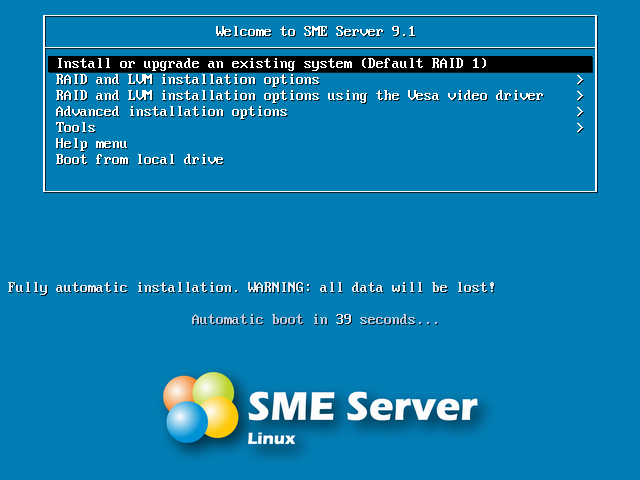
\includegraphics[width=\textwidth]{capitulo02/00.png}
\end{figure}

Por defecto, el servidor usará los discos disponibles en modo RAID 1. Sin embargo podemos usar la segunda opción para elegir manualmente el nivel de RAID que queremos. Si seleccionamos 'Advanced installation options', nos llevará a un instalador gráfico en el que tendremos alguna opción más, como instalar el sistema en volúmenes de alacenamiento en la red, como iSCSI.

\begin{figure}[H]
    \centering
    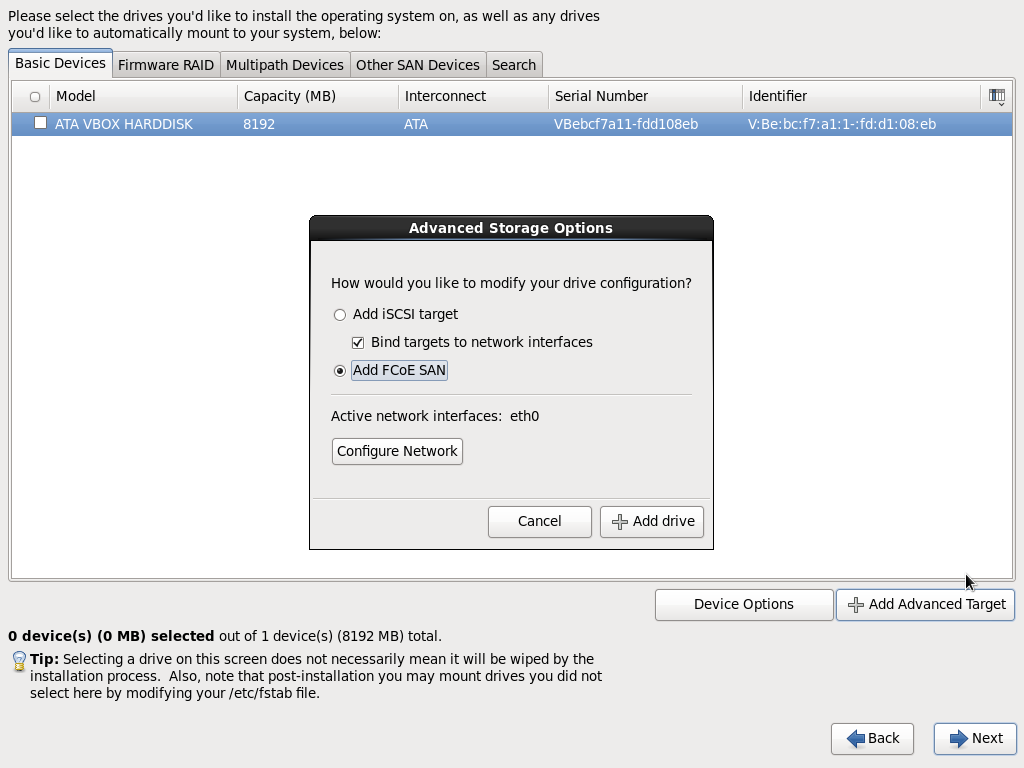
\includegraphics[width=\textwidth]{capitulo02/31instAv.png}
\end{figure}

La instalación borrará los discos completamente. No tenemos la opción de elegir el particionado manualmente. Por ejemplo, una máquina con 5 discos en RAID 5, este es el particionado que obtenemos tras la instalación:

\begin{figure}[H]
    \centering
    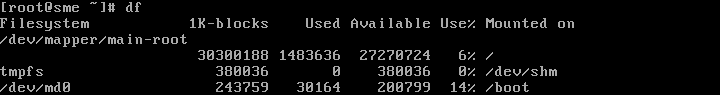
\includegraphics[width=\textwidth]{capitulo02/32raid5.png}
\end{figure}

En esta parte de la instalación solo podemos elegir el lenguaje y el tipo de teclado que vamos a utilizar. Cuando el sistema termina de instalarse, se reinicia y nos pregunta por varios aspectos de la configuración.

\section{Configuración inicial}

La primera vez que iniciamos la máquina tras instalar SME server tenemos que configurar el sistema. Nos pregunta por los siguientes parámetros:

\begin{itemize}
\item Contraseña del sistema.
\item Nombre del dominio y del sistema.
\item Configuración de la interfaz de red interna, asignación de IP y máscara.
\item Elegir el modo de operación del servidor.
\begin{figure}[H]
    \centering
    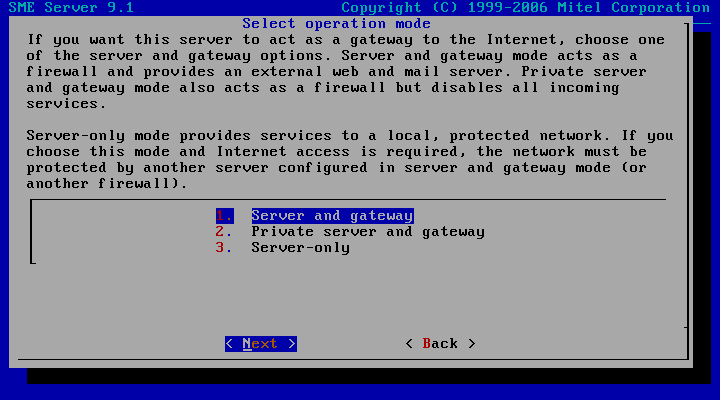
\includegraphics[width=\textwidth]{capitulo02/18.png}
\end{figure}
Tenemos 3 opciones:
\begin{itemize}
\item[\textbf{-}] \textbf{Server and gateway}. El servidor provee los servicios como email, web e intercambio de archivos e impresoras a la red interna y actúa como router y gateway entre la red interna e Internet. También actúa de firewall.
\item[\textbf{-}] \textbf{Private server and gateway}. Esta opción se diferencia del anterior en que los servicios que proporciona el servidor no son accesibles desde la red externa, y además el firewall contiene reglas adicionales.
\item[\textbf{-}] \textbf{Server-only mode}. En este modo, el servidor sólo se conecta a la red interna y ofrece los servicios ahí.
\end{itemize}
\item Configuración de la interfaz de red externa. Debemos decirle de qué manera se va a conectar a internet.
\begin{figure}[H]
  \centering
  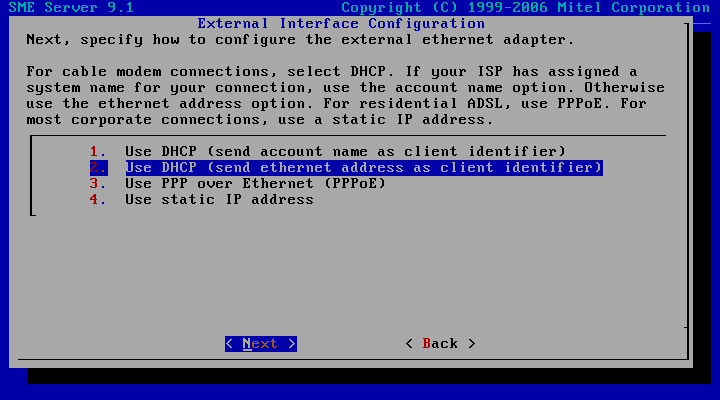
\includegraphics[width=\textwidth]{capitulo02/21.png}
\end{figure}
\item Configuración de un servicio de DNS dinámico.
\begin{figure}[H]
    \centering
    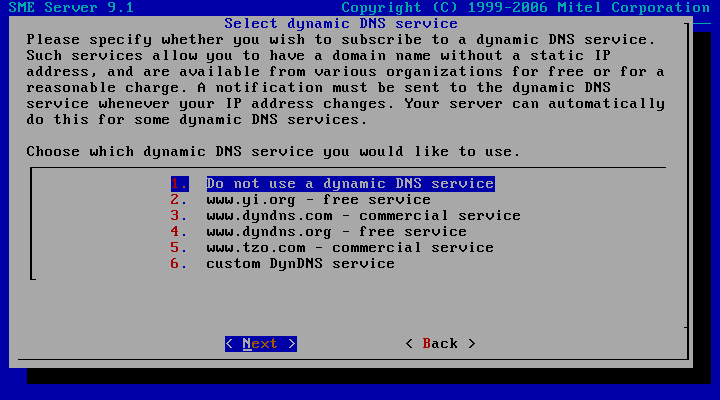
\includegraphics[width=\textwidth]{capitulo02/22.png}
\end{figure}
\item Configuración del DHCP para la red interna.
\item Por último nos pregunta si queremos usar otro servidor DNS que ya existiera en nuestra red interna.
\end{itemize}

En cuanto terminamos la configuración inicial ya tenemos un servidor completamente funcional ofreciendo distintos servicios. Vamos a ver sus características por defecto y las formas que tenemos de modificarlos.

\section{Modos de administración}

Existen varios modos distintos de adminstrar el SME server.

\subsection{Consola de root de Linux}

Al arrancar el sistema, accedemos con el usuario "root" y la contraseña de administración. Esto nos proporciona un acceso al sistema operativo mediante la terminal de Linux.\\

\begin{figure}[H]
    \centering
    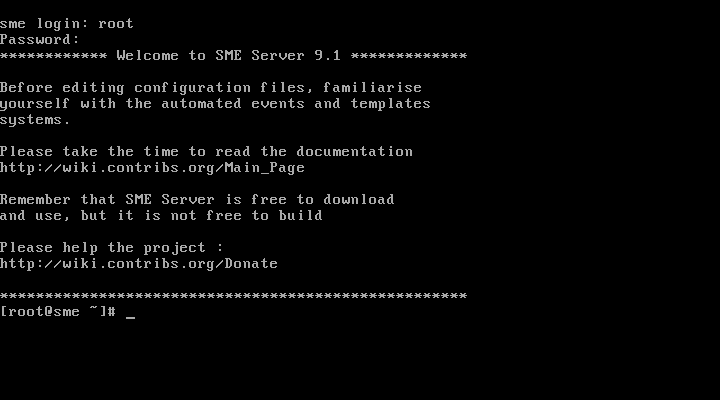
\includegraphics[width=\textwidth]{capitulo02/29.png}
\end{figure}

\subsection{Consola del servidor}

Al arrancar el sistema, accedemos con el usuario usuario "admin" y la contraseña de administración. También se puede acceder desde la consola de root, escribiendo "console".\\

\begin{figure}[H]
    \centering
    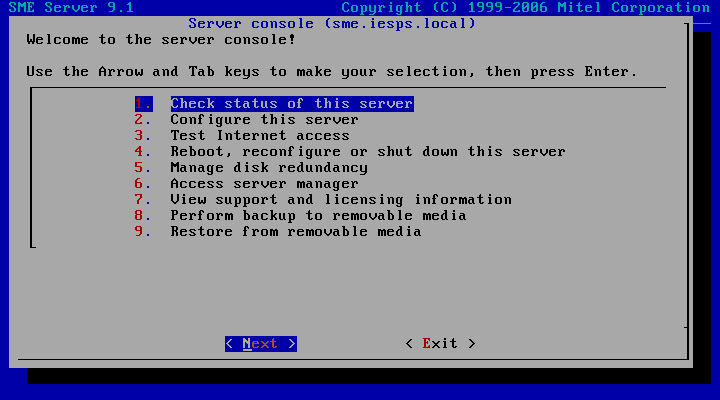
\includegraphics[width=\textwidth]{capitulo03/00.png}
\end{figure}

Tiene varias opciones
\begin{enumerate}
 \item \textbf{Check status of this server}: muestra el tiempo que ha estado en marcha el servidor.
\item \textbf{Configure this server}: nos lleva otra vez a través de las pantallas de la configuración inicial por si queremos cambiar algo.
\item \textbf{Test internet access}: prueba el acceso a internet mandando datos a contribs.org.
\item \textbf{Reboot, reconfigure or shut down this server}: reiniciar, reconfigurar o apagar el servidor.
\item \textbf{Manage disk redundancy}: muestra el estado de los discos y permite administrar el tipo de RAID. En nuestro caso solo hay un disco instalado... Parece que ha hecho 2 particiones (MIRAR).
\item \textbf{Access server manager}: permite acceder a la interfaz de administración web server-manager desde el mismo servidor usando el navegador en modo texto ELinks.
\item \textbf{View Support and licensing information}: ver la licencia (GNU GPL) e información sore cómo contactar con contribs.org para el soporte.
\item \textbf{Perform backup to removable media}: permite hacer un backup del estado actual del servidor en una unidad USB. La imagen se comprime en un archivo .tgz.
\item \textbf{Restore from removable media}: permite recuperar una imagen del servidor anteriormente guardada en una unidad USB.
\end{enumerate}

\subsection{Aceso remoto}
Podemos acceder a estos dos modos de administración desde otro PC a través de SSH, pero está desactivado por defecto:

\begin{figure}[H]
    \centering
    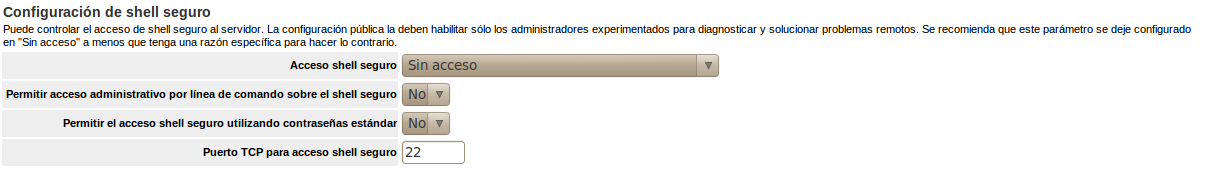
\includegraphics[width=\textwidth]{capitulo03/ssh00.png}
\end{figure}

En esta práctica permitiremos el acceso por SSH desde las redes locales para una administración más sencilla. Una vez activado, tendremos disponibles las dos primeras formas de administración que hemos explicado, dependiendo de si nos conectamos como 'root' o como 'admin'. SME server permite también el acceso mediante PPTP para la administración.

\subsection{Interfaz web server-manager}

SME Server provee una interfaz web de administración. Se accede desde el navegador de cualquier ordenador de la red interna con cualquiera de las siguientes URL:

\begin{itemize}
  \item https://sme/server-manager
  \item https://192.168.0.254/server-manager
\end{itemize}

\begin{figure}[H]
    \centering
    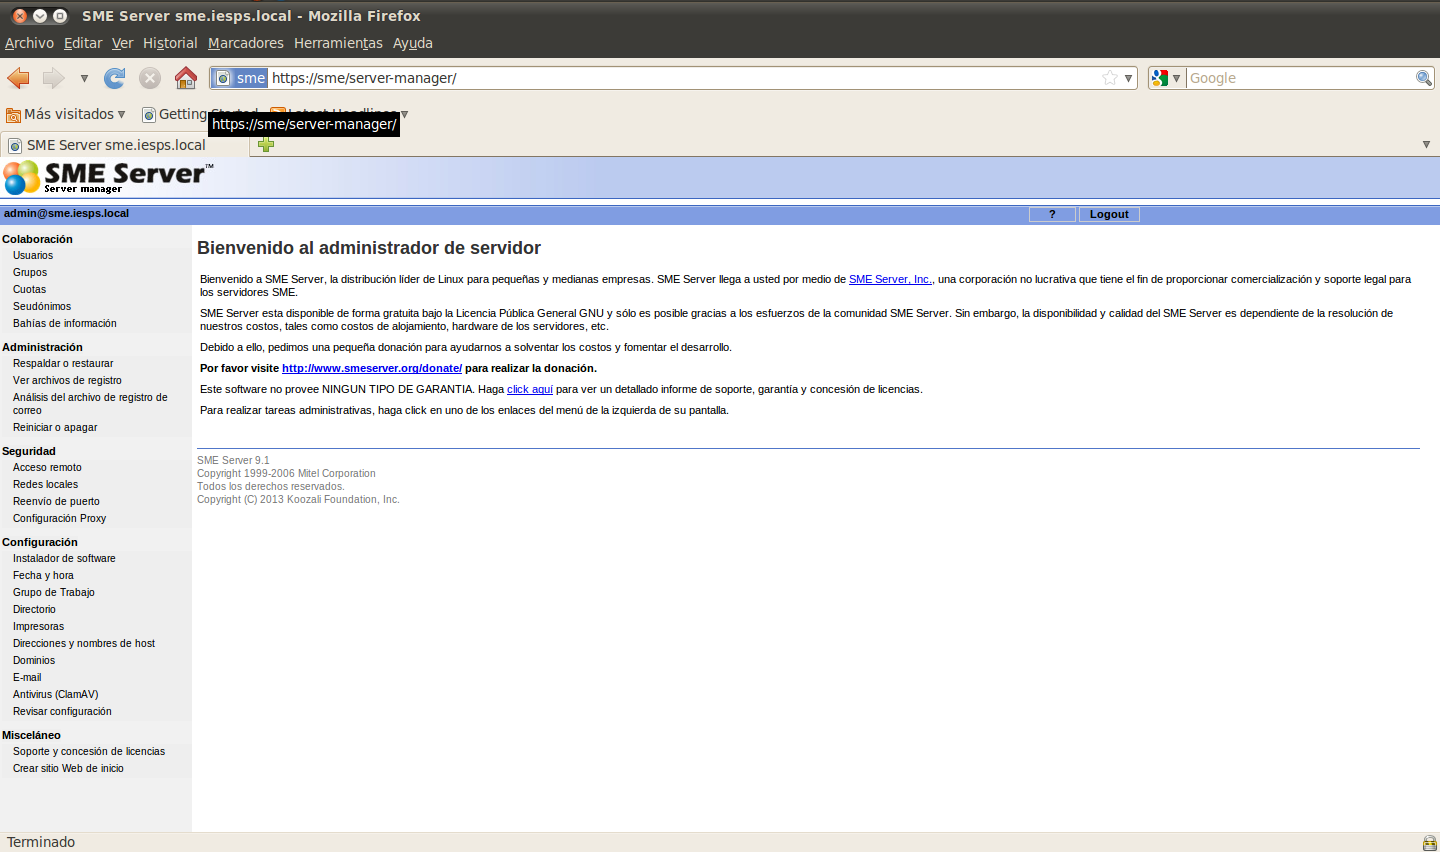
\includegraphics[width=\textwidth]{capitulo03/11.png}
\end{figure}

\section{Servicios y caracerísticas}

\begin{itemize}
\item Actúa como gateway, y proporciona un firewall, que luego veremos en más detalle. También actúa como servidor DNS.
\item Servidor Web.
\item Cuentas de usuario y grupos. Cada cuenta de usuario en SME server incluye una cuenta de email y un área de almacenamiento, en principio sin límite máximo, aunque se puede establecer.
\item Servidor de Directorio Activo.
\item Email. Existe la opción de reenviar los emails de un usuario o grupo a una cuenta externa. Se pueden crear varios pseudónimos para cada cuenta de email. SME nos da la opción de redirigir estos emails a una cuenta externa.
\item Almacenamiento. El área de almacenamiento de cada usuario está disponible con Samba. Aparte de esto, se pueden establecer bahías de información, o i-bays, que son directorios compartidos en el disco duro sobre los que podemos establecer fácilmente el control de acceso y los podemos proteger con contraseña.

\begin{figure}[H]
    \centering
    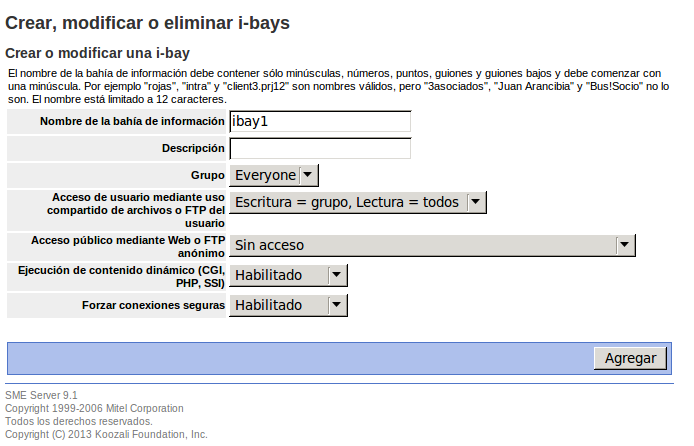
\includegraphics[width=\textwidth]{capitulo02/33.png}
\end{figure}

Los contenidos se encuentran en \lstinline!/home/e-smith/files/ibays/nombre_ibay/files!.
\end{itemize}


%\chapter{Configuración por defecto}
%
En cuanto terminamos la configuración inicial ya tenemos un servidor completamente funcional ofreciendo distintos servicios. Vamos a ver sus características por defecto y las formas que tenemos de modificarlos.

\section{Modos de administración}

Existen varios modos distintos de adminstrar el SME server.

\subsection{Consola de root de Linux}

Al arrancar el sistema, accedemos con el usuario "root" y la contraseña de administración. Esto nos proporciona un acceso al sistema operativo mediante la terminal de Linux.\\

\begin{figure}[H]
    \centering
    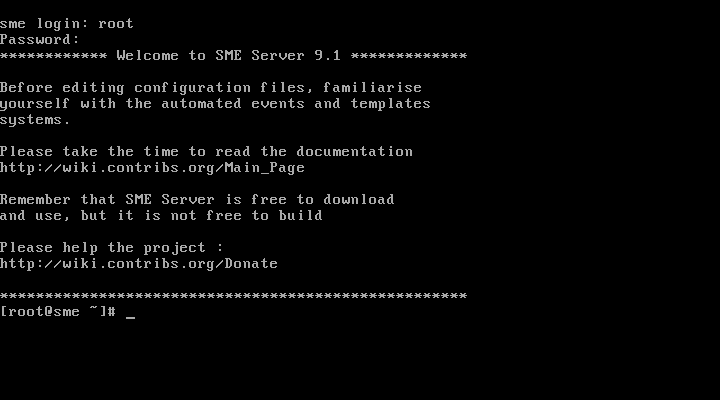
\includegraphics[width=\textwidth]{capitulo02/29.png}
\end{figure}

\subsection{Consola del servidor}

Al arrancar el sistema, accedemos con el usuario usuario "admin" y la contraseña de administración. También se puede acceder desde la consola de root, escribiendo "console".\\

\begin{figure}[H]
    \centering
    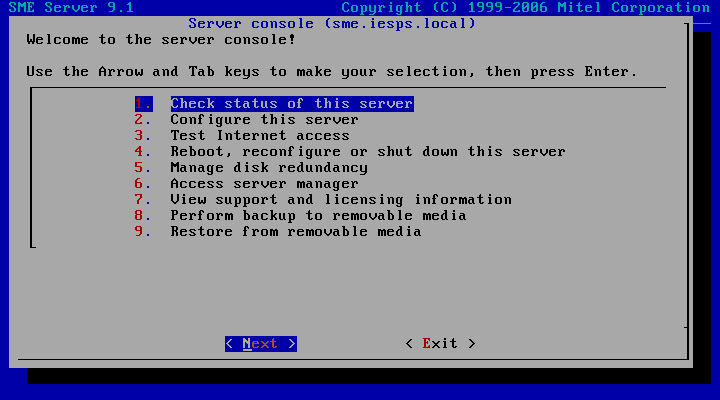
\includegraphics[width=\textwidth]{capitulo03/00.png}
\end{figure}

Tiene varias opciones
\begin{enumerate}
 \item \textbf{Check status of this server}: muestra el tiempo que ha estado en marcha el servidor.
\item \textbf{Configure this server}: nos lleva otra vez a través de las pantallas de la configuración inicial por si queremos cambiar algo.
\item \textbf{Test internet access}: prueba el acceso a internet mandando datos a contribs.org.
\item \textbf{Reboot, reconfigure or shut down this server}: reiniciar, reconfigurar o apagar el servidor.
\item \textbf{Manage disk redundancy}: muestra el estado de los discos y permite administrar el tipo de RAID. En nuestro caso solo hay un disco instalado... Parece que ha hecho 2 particiones (MIRAR).
\item \textbf{Access server manager}: permite acceder a la interfaz de administración web server-manager desde el mismo servidor usando el navegador en modo texto ELinks.
\item \textbf{View Support and licensing information}: ver la licencia (GNU GPL) e información sore cómo contactar con contribs.org para el soporte.
\item \textbf{Perform backup to removable media}: permite hacer un backup del estado actual del servidor en una unidad USB. La imagen se comprime en un archivo .tgz.
\item \textbf{Restore from removable media}: permite recuperar una imagen del servidor anteriormente guardada en una unidad USB.
\end{enumerate}

\subsection{Aceso remoto}
Podemos acceder a estos dos modos de administración desde otro PC a través de SSH, pero está desactivado por defecto:

\begin{figure}[H]
    \centering
    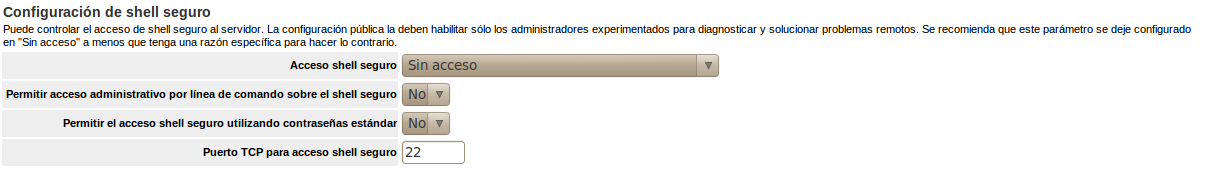
\includegraphics[width=\textwidth]{capitulo03/ssh00.png}
\end{figure}

En esta práctica permitiremos el acceso por SSH desde las redes locales para una administración más sencilla. Una vez activado, tendremos disponibles las dos primeras formas de administración que hemos explicado, dependiendo de si nos conectamos como 'root' o como 'admin'. SME server permite también el acceso mediante PPTP para la administración.

\subsection{Interfaz web server-manager}

SME Server provee una interfaz web de administración. Se accede desde el navegador de cualquier ordenador de la red interna con cualquiera de las siguientes URL:

\begin{itemize}
  \item https://sme/server-manager
  \item https://192.168.0.254/server-manager
\end{itemize}

\begin{figure}[H]
    \centering
    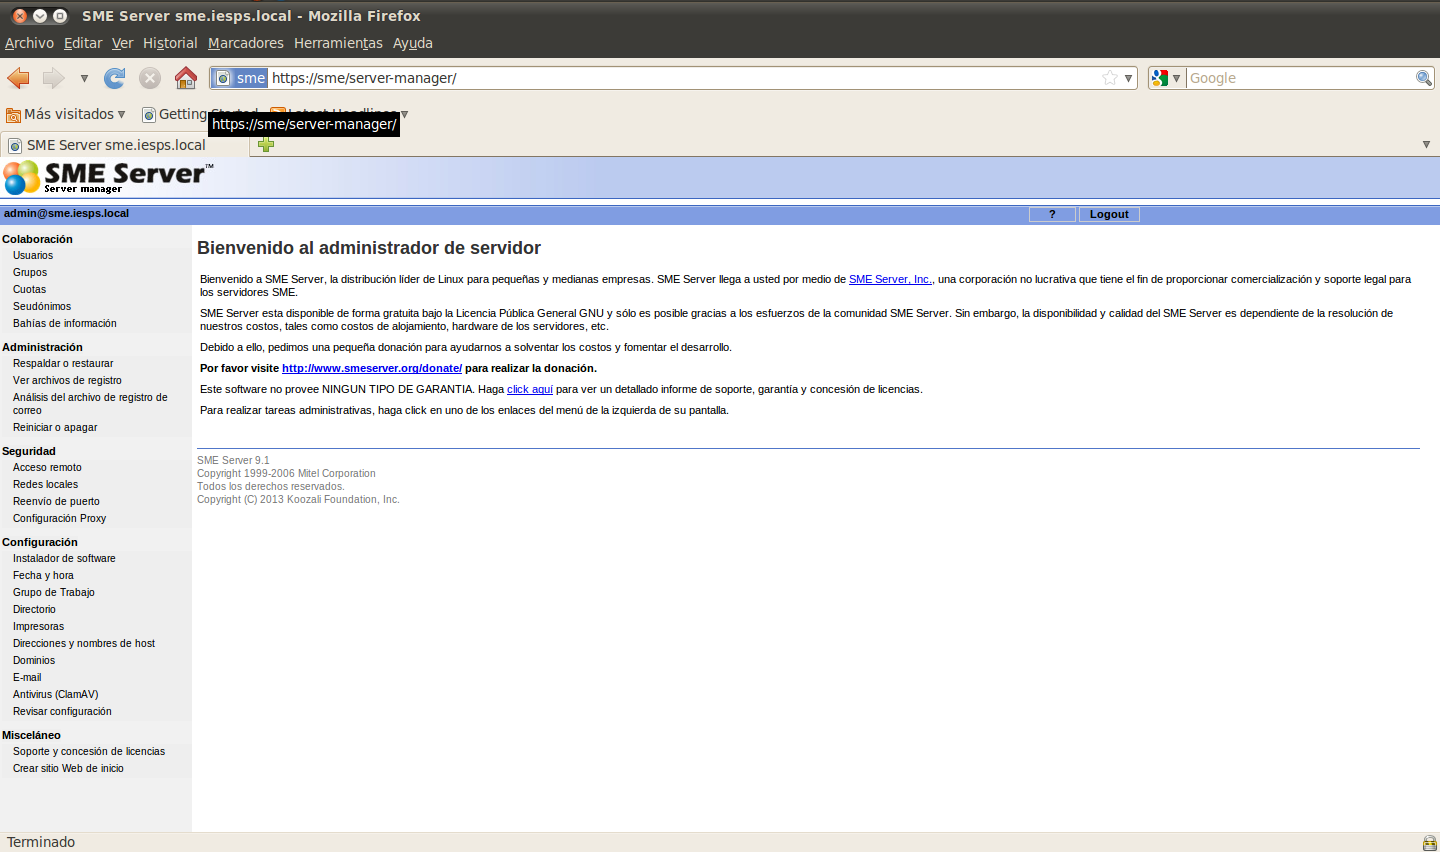
\includegraphics[width=\textwidth]{capitulo03/11.png}
\end{figure}
\newpage 
\section{Servicios y caracerísticas}

\subsection{Usuarios}

Las cuentas de usuario en SME server incluyen cuentas de email y áreas de almacenamiento separadas y protegidas por contraseña.

-> Opcion de reenvio para los emails

-> Como cambiar la password desde el navegador web

-> The user group function serves two purposes in the SME Server: it permits email to be sent conveniently to a group of users, and it allows the system administrator to associate groups of users with a single information bay (i-bay).

-> By default, there is no size limit on the files a user may store on the server nor the amount of email that can be received. However, if you wish to limit the disk space a particular user account can use, you may do so on the " Quotas " panel in the server-manager.

\subsection{email}

Configuración general

\begin{figure}[H]
    \centering
    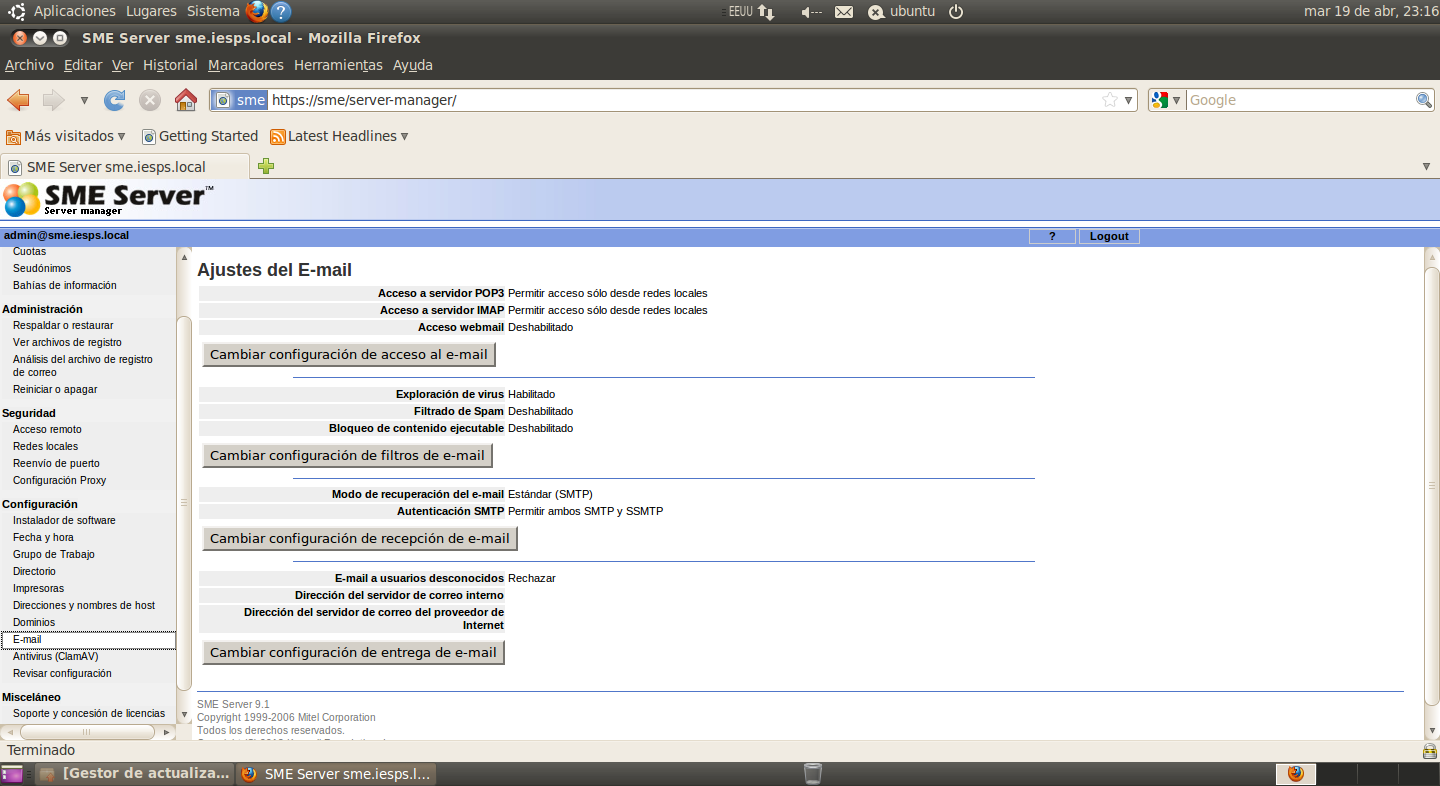
\includegraphics[width=\textwidth]{capitulo03/13email.png}
\end{figure}

\subsection{Almacenamiento, i-bays}

\subsection{DNS}

...




\chapter{Herramientas LAT}
Las herramientas LAT (Lazy Admin Tools en inglés) son una serie de scripts diseñados para automatizar ciertas tareas de administración en SME server. En este momento las herramientas disponibles son:\\

\begin{longtable}{ c | l }
  \textbf{Comando} & \textbf{Descripción} \\\hline
  lat-users & Añadir/borrar usuarios (y sus directorios)\\
  lat-groups & Añadir/borrar grupos\\
  lat-pseudonyms & Añadir/borrar pseudónimos de email para usuarios indivuduales\\
  lat-ibays & Añadir/borrar ibays (y sus directorios)\\
  lat-quota & Determinar la cuota de uso de disco para usuarios individuales\\
  lat-procmail & Activar o desactivar procmail (herramienta de filtrado de email) \\
  & para usuarios individuales\\
  lat-hosts & Añadir o quitar nombres de hosts\\
  lat-domains & Crear dominios virtuales\\
  lat-pptp & Activar o desactivar acceso pptp para usuarios individuales\\
  lat-dump & Crear archivos de input para las herramientas anteriores\\
  lat-shadow & Transferir una contraseña encriptada desde un servidor SME a otro\\
\end{longtable}

Cada una de ellas tiene su entrada correspondiente en el manual. A continuación instalaremos las herramientas LAT y como ejemplo de su utilización usaremos lat-users para crear varios usuarios.

\section{Instalación}

Las herramientas LAT se encuentran en el repositorio 'smecontribs'. Para instalarlas junto a los paquetes necesarios usaremos el siguiente comando:

\begin{lstlisting}
yum install --enablerepo=smecontribs smeserver-lazy_admin_tools smeserver-userpanel smeserver-mailsorting
\end{lstlisting}

Tras instalarlo, nos advierte de que debemos reiniciar:

\begin{lstlisting}
signal-event post-upgrade; signal-event reboot
\end{lstlisting}

\section{lat-users}
lat-users permite crear o eliminar cuentas de usuario. Su funcionalidad es equivalente a la opción 'User accounts' en la interfaz web, pero se puede ejecutar desde la línea de comandos, con lo que puede ser utilizado en scripts.\\

Siempre que queramos crear usuarios deberemos usar esta herramienta o bien la interfaz web, nunca los comandos \lstinline!adduser! o \lstinline!useradd! de Linux, ya que SME Server posee una base de datos propia de todos los usuarios y grupos, que no se actualiza si no se añaden correctamente.

\subsection{Sintaxis}
Depende de cómo lo queramos usar, la sintaxis es una de las siguientes:
\begin{lstlisting}
lat-users -a [-p] -c "user | first | last | password | department | company | street | city | tel | forward | email | uid | group1 [| group2..]"
\end{lstlisting}
\begin{lstlisting}
lat-users -a [-p] -i /ruta/a/users.list
\end{lstlisting}
\begin{lstlisting}
lat-users -d [-f] -c "usuario" 
\end{lstlisting}
\begin{lstlisting}
lat-users -d [-f] -i /ruta/a/users.list
\end{lstlisting}

\subsection{Opciones}
\begin{longtable}{p{0.43\textwidth} | p{0.48\textwidth} }
\textbf{Comando} & \textbf{Descripción} \\\hline
\lstinline!-a, --add! & Añade una cuenta de usuario\\\hline
\lstinline!-n! & Crea pseudónimos de email: nombre.apellido y nombre\_apellido\\\hline
\lstinline!-c "Args.", --command-line="Args."! & Recibe argumentos de la línea de comandos. La lista de argumentos se muestra debajo\\\hline
\lstinline!-d, --delete! & Borra una cuenta de usuario. Acepta las wildcards * y ?\\\hline
\lstinline!-f! & Fuerza el borrado de usuarios, no pregunta confirmación.\\\hline
\lstinline!-h! & Muestra la ayuda.\\\hline
\lstinline!-i=ARCHIVO, --input-file=ARCHIVO! & Obtiene la información para la creación o borrado de usuarios desde un archivo.\\\hline
\lstinline!-p, --passwords! & Genera contraseñas aleatorias para los nuevos usuarios y las escribe en ./passwords.new.
\end{longtable}

La lista de argumentos aceptados, en orden, es la siguiente:\\

\begin{longtable}{p{0.15\textwidth} | p{0.76\textwidth} }
\textbf{Argumento} & \textbf{Descripción}\\\hline
\lstinline!user! & Nombre de usuario de Linux. Sólo puede contener letras minúsculas, números, puntos y barras bajas. Debe empezar con una letra minúscula. Las wildcards * y ? se pueden usar para eliminar usuarios\\\hline
\lstinline!first! & Nombre\\\hline
\lstinline!last! & Apellido\\\hline
\lstinline!password! & Contraseña (en texto plano)\\\hline
\lstinline!department! & Departamento\\\hline
\lstinline!company! & Compañía\\\hline
\lstinline!street! & Dirección: calle y número\\\hline
\lstinline!city! & Dirección: código postal y ciudad \\\hline
\lstinline!tel! & Número de teléfono \\\hline
\lstinline!forward! & Tipo de entrega de email. Puede ser 'local' , 'forward' o 'both'\\\hline
\lstinline!email! & Dirección a la que reenviar el email \\\hline
\lstinline!uid! & ID de usuario. Si se omite, se genera automáticamente \\\hline
\lstinline!group(s)! & Grupos a los que el usuario debe ser añadido. Si no existe el grupo, se creará \\
\end{longtable}

Los campos \lstinline!user!, \lstinline!first! y \lstinline!last! son obligatorios.

\subsection{Ejemplos}
En el archivo /usr/doc/lazy-admin-tools/example.users tenemos varios ejemplos de sintaxis válidas para la opción \lstinline!-c!
\begin{figure}[H]
    \centering
    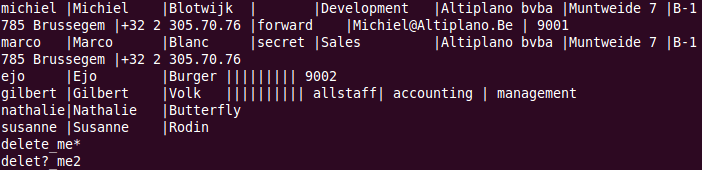
\includegraphics[width=\textwidth]{lat/us00-archivoDeEjemplo.png}
    \caption{Ejemplos de creación y borrado de usuarios}
\end{figure}

Las líneas primera y segunda en realidad serían una única, pero se corta. Lo mismo pasa con las líneas tercera y cuarta. Las dos últimas sólo son válidas para el borrado de usuarios.\\

Si queremos crear una lista completa de usuarios como por ejemplo los que usamos en clase, desde alu01 hasta alu40, tenemos varias alternativas. La primera sería escribir un script que los vaya creando uno a uno usando \lstinline!lat-users -a!:

\begin{lstlisting}
#!/bin/bash

for I in $(seq -w 1 1 40)
do
    lat-users -a -c "alu$I|Alumno|$I|alu$I| | | | | | | | |asir2d"
done
\end{lstlisting}

Los grupos alu01, ..., alu40 se crean automáticamente y se asignan como grupo primario de los correspondientes usuarios.\\

Otra opción es hacer un shell script que escriba un archivo como el users.list que hemos visto anteriormente, y usar luego \lstinline!lat-users -a -i ./users.list!:

\begin{lstlisting}
#!/bin/bash

for I in $(seq -w 1 1 40)
do
    echo "alu$I|Alumno|$I|alu$I| | | | | | | | |asir2d" >> ./users.list  
done
\end{lstlisting}

Puede ocurrir que hayamos escrito el comando erróneamente y se haya creado un usuario o un grupo 'a medias', de manera que no existirá como tal pero seguirá estando en la base de datos, con lo cual no podremos crearlo otra vez. Para eliminar completamente un usuario o grupo en estos casos usaremos:

\begin{lstlisting}
signal-event user-delete usuario
db accounts delete usuario
\end{lstlisting}

O bien

\begin{lstlisting}
signal-event group-delete grupo
db accounts delete grupo
\end{lstlisting}

Un script que viene bien para borrar completamente todos los usuarios añadidos en el ejemplo:

\begin{lstlisting}
#!/bin/bash

lat-users -d -f -c "alu*"

for I in $(seq -w 1 1 40)
do
    signal-event user-delete alu$I
    db accounts delete alu$I
done

signal-event reboot
\end{lstlisting}


\chapter{Arquitectura del SME Server}
%http://distro.ibiblio.org/smeserver/contribs/gordonr/devguide/html/c1115.htm
%http://www.sme-server.de/download/Howtos/Customizing_SME.html
%https://wiki.contribs.org/SME_Server:Documentation:Developers_Manual

La arquitectura interna del SME Server se basa en cuatro componentes:

\begin{itemize}
\item Interfaces de administración, tanto por consola como web.
\item Bases de datos de configuración.
\item El sistema de templates, que es usado para generar archivos de configuración.
\item Eventos y acciones.
\end{itemize}

Cuando un usuario configura alguno de los aspectos del servidor, la máquina configura automáticamente las aplicaciones que son relevantes a ese cambio. Esto se realiza en varios pasos:
\begin{itemize}
\item La interfaz de usuario cambia valores en las bases de datos de configuración. En estas bases de datos se almacena información que describe el estado del sistema, como las asignaciones de direcciones IP, los nombres de dominio, las cuentas de usuario...
\item Después de haber cambiado estos valores, la interfaz de usuario envía una señal de evento para realizar los cambios en las aplicaciones. Por ejemplo, si hacemos cambios en la configuración del email, el evento que se señala es el 'email-update'. Estos eventos son colecciones de scripts, que se ejecutan en un orden determinado para producir las modificaciones deseadas.
\item Estos scripts actualizan los ficheros de configuración de las aplicaciones. Los generan usando las templates, que no son más que plantillas usadas para este propósito. Los scripts de actualización leen las bases de datos de configuración, de manera que los nuevos archivos generados contienen nuestras últimas modificaciones.
\item Por último las aplicaciones son avisadas de que su configuración ha sido cambiada, por lo que releen los archivos o se reinician, según convenga.
\end{itemize}

Aquí tenemos una imagen que describe este proceso:

\begin{figure}[H]
    \centering
    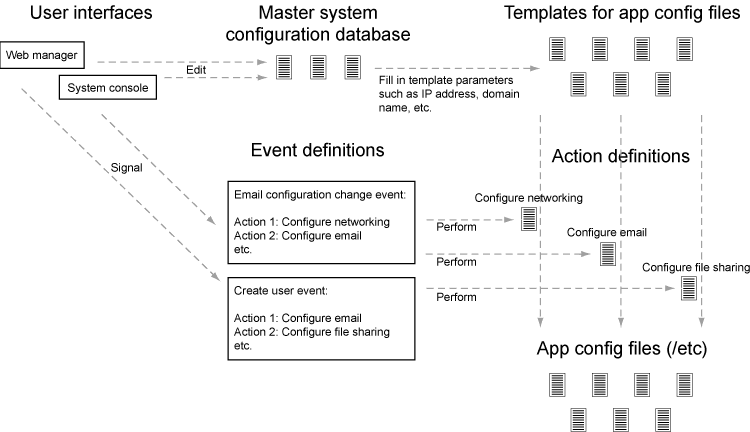
\includegraphics[width=\textwidth]{arquitectura/Sme-server-architecture.png}
%    \caption{Arquitectura interna del SME server}
\end{figure}

\section{Bases de datos de configuración}
Todos los parámetros de configuración que son modificables por el usuario son almacenados aquí. Las entradas pueden ser de dos tipos:
\begin{itemize}
\item Simples: constan de un par clave/valor.
\begin{figure}[H]
    \centering
    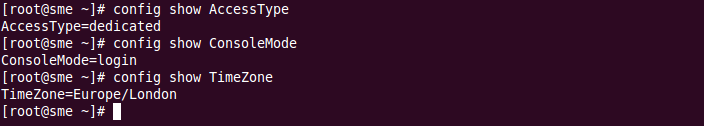
\includegraphics[width=\textwidth]{arquitectura/01.png}
%    \caption{Entradas simples}
\end{figure}
\item Complejas: constan de una clave, un tipo y una colección de pares propiedad/valor.
\begin{figure}[H]
    \centering
    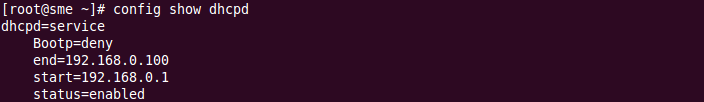
\includegraphics[width=\textwidth]{arquitectura/02.png}
%    \caption{Entradas complejas}
\end{figure}
\end{itemize}

\subsection{Acceso a las bases de datos}

\begin{itemize}
\item \textbf{Acceso mediante la línea de comandos}
\end{itemize}
El comando para acceder a los datos de las bases de datos de configuración es \lstinline!db!. Podemos ver una pequeña ayuda tecleando \lstinline!db! sin más:
\begin{figure}[H]
    \centering
    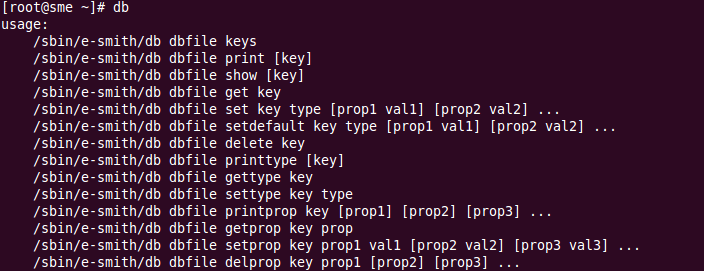
\includegraphics[width=\textwidth]{arquitectura/03.png}
\end{figure}

Las bases de datos existentes son \lstinline!accounts!, \lstinline!networks!, \lstinline!configuration!, \lstinline!domains! y \lstinline!hosts!. Además, tenemos el comando \lstinline!config show!, que es un alias para \lstinline!db configuration show!.

\begin{figure}[H]
    \centering
    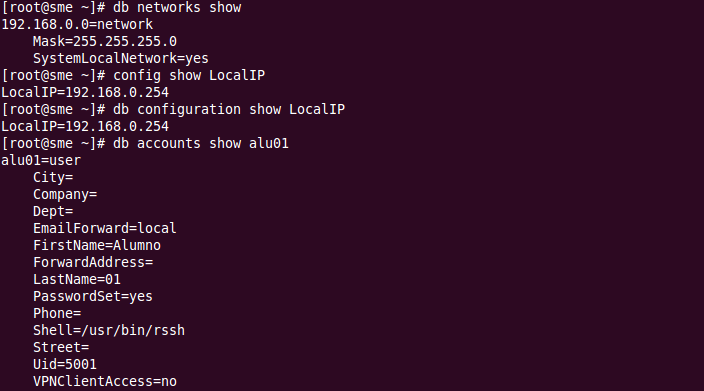
\includegraphics[width=\textwidth]{arquitectura/04.png}
\end{figure}

\begin{itemize}
\item \textbf{Acceso desde un script de Perl}
\end{itemize}

SME Server incorpora una API para Perl para acceder a las bases de datos de configuración. Para ver ayuda y ejemplos, podemos acceder a la documentación usando el comando \lstinline!perldoc!:

\begin{lstlisting}
  perldoc esmith::ConfigDB
  perldoc esmith::AccountsDB
  perldoc esmith::HostsDB
  perldoc esmith::NetworksDB

  perldoc esmith::DB
\end{lstlisting}

%Esto está comentado
\begin{comment}
Script para consultar el usuario admin:

\begin{lstlisting}[language=Perl,style=perlo]
#!/usr/bin/perl -w
  
use esmith::AccountsDB;

my $db = esmith::AccountsDB->open or die "No se puede abrir la BD Accounts\n";

my $admin = $db->get("admin") or die "No existe la cuenta admin en la BD ACcounts\n";

print $admin->show();
\end{lstlisting}
\end{comment}
%%%%%%%%%%%%%%%%%%%

%----------------------------------------------------------
%
%         ACCIONES Y EVENTOS
%
%----------------------------------------------------------
\section{Acciones y eventos}

\subsection{Acciones}

Una acción es un programa que ejecuta una única tarea, como editar un archivo de configuración o reconfigurar un servicio. Las acciones son llamadas marcando un evento, nunca directamente. Están en el directorio \lstinline!/etc/e-smith/events/actions!.

\begin{figure}[H]
    \centering
    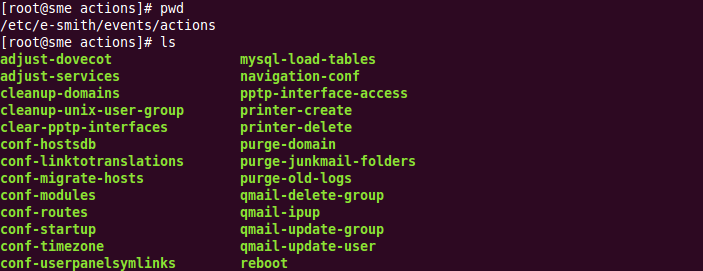
\includegraphics[width=\textwidth]{arquitectura/05listaActions.png}
\end{figure}

\subsection{Eventos}

Los eventos son un mecanismo que permite al sistema ejecutar una serie de acciones en respuesta a un cambio. Están asociados a una lista de acciones que se ejecutan en un orden determinado. Se encuentran en la carpeta \lstinline!/etc/e-smith/events!\\

Por ejemplo, en el caso de un cambio de la dirección IP externa, se llamaría al evento \lstinline!ip-change!. Este evento se compone de lo siguiente:

\begin{figure}[H]
    \centering
    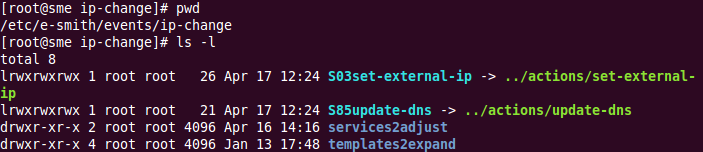
\includegraphics[width=\textwidth]{arquitectura/06eventoIp.png}
\end{figure}

\begin{itemize}
\item Enlaces simbólicos a dos acciones, una que escribe la nueva IP externa en la base de datos \lstinline!configuration! y otra que actualiza el servicio de DNS dinámico que tuviéramos configurado con la nueva IP de nuestra máquina. El prefijo que llevan los links sirve para establecer en qué orden se ejecutarán. Este es el cuerpo del script que cambia la IP externa:
\end{itemize}

\begin{figure}[H]
    \centering
    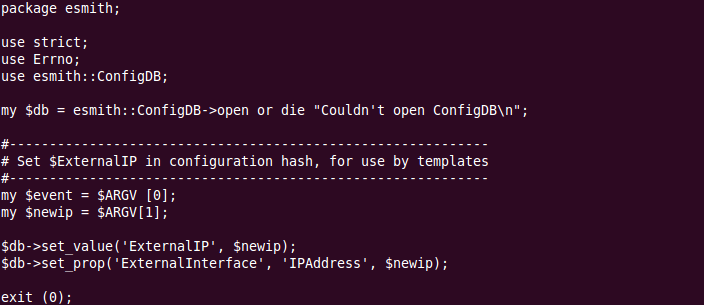
\includegraphics[width=\textwidth]{arquitectura/07set-external-ip.png}
\end{figure}

Aquí podemos ver cómo se usa el API de Perl para acceder a la base de datos \lstinline!configuration! y cambiar valores. Casi todas las acciones son llamadas siempre con 2 argumentos: el nombre del evento que las ha llamado y el nuevo valor que se va a asignar. La IP externa del equipo es guardada en 2 registros diferentes de esta base de datos, por razones de compatibilidad con versiones anteriores de SME server:

\begin{figure}[H]
    \centering
    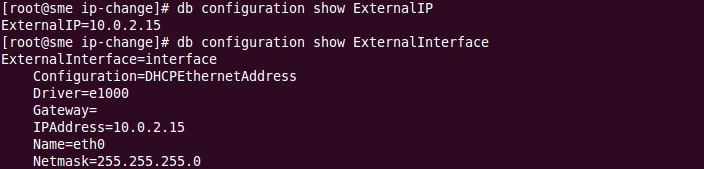
\includegraphics[width=\textwidth]{arquitectura/08extInterfaceEnBD.png}
\end{figure}

\begin{itemize}

\item Acciones implícitas. La mayoría de eventos contienen dos tareas comunes: expandir los templates necesarios y reajustar los servicios implicados. Para ello se ejecutan las acciones \lstinline!generic_template_expand! y \lstinline!adjust-services!, cuyo código se encuentra en \lstinline!/etc/e-smith/events/actions!. Los subdirectorios que encontramos en la carpeta de nuestro evento son usados por estas dos acciones:

\begin{itemize}

\item[-] Directorio \lstinline!services2adjust!, para la acción \lstinline!adjust-services!. Contiene links de los servicios que se tienen que reajustar y la acción que se debe efectuar sobre ellos.

\begin{figure}[H]
    \centering
    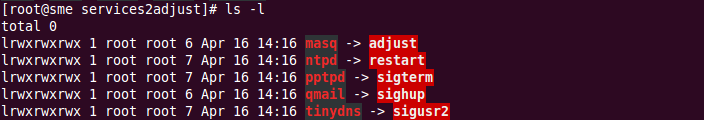
\includegraphics[width=\textwidth]{arquitectura/09services2adjust.png}
\end{figure}

\item[-] Directorio \lstinline!templates2expand!. Lista de los archivos de configuración que tienen que volver a ser regenerados desde las plantillas.

\begin{figure}[H]
    \centering
    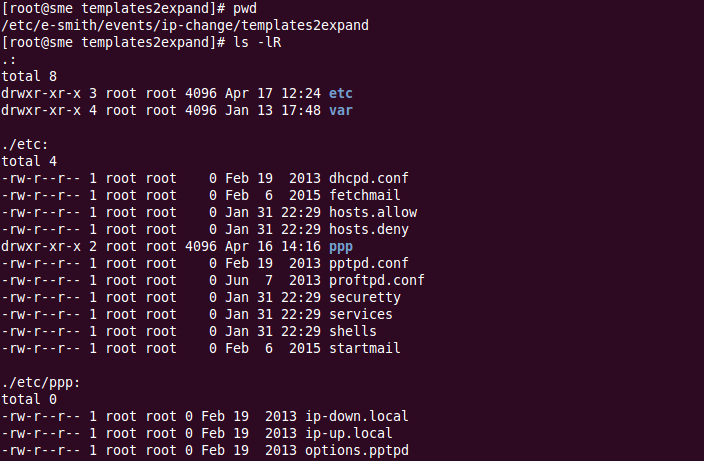
\includegraphics[width=\textwidth]{arquitectura/10templates2expand.png}
\end{figure}
\end{itemize}
\end{itemize}

Por defecto, la acción \lstinline!generic_template_expand! se ejecua con prioridad S05, y la acción \lstinline!adjust-services! con S90. Por ello se recomienda que las acciones propias que queramos incluir estén entre S10 y S80. Sabiendo esto podemos comprender el orden en el que se ejecutan las acciones en nuestro ejemplo, el evento de cambio de IP externa:
\begin{enumerate}
\item Se cambia el valor de IP externa en la base de datos de configuración.
\item Se actualizan los archivos de configuración de los servicios y programas implicados.
\item Si tenemos configurado servicio de DNS dinámico, se actualiza (se advierte al servidor de nuestro cambio de IP).
\item Se reconfiguran todos los servicios con la nueva IP.
\end{enumerate}

\subsection{Señalar un evento}
Para ejecutar todas las acciones de un evento usamos el comando \lstinline!signal-event!, seguido del nombre del evento. Este comando además escribe todo el output en el log del sistema \lstinline!messages!.

\begin{lstlisting}
  signal-event ip-change 216.58.210.35
\end{lstlisting}

El comando \lstinline!signal-event! no suele tener más argumentos que el nombre del evento, ya que en general se prefiere hacer los cambios en los archivos de configuración antes de llamar al evento.

%%%%%
\begin{comment}
\subsection{Eventos importantes}

\begin{longtable}{p{0.15\textwidth} |p{0.15\textwidth} | p{0.61\textwidth} }
  \textbf{Evento} & \textbf{Argumento} & \textbf{Descripción}\\\hline
  \lstinline!aaa! & - & bbb\\
\end{longtable}
\end{comment}
%%%%%

%----------------------------------------------------------
%
%         TEMPLATES
%
%----------------------------------------------------------

\section{Templates}

El sistema de templates (plantillas) presente en SME server sirve para generar los archivos de configuración de las aplicaciones. Proporciona un método uniforme para cambiar estos archivos, sin tener que preocuparnos de la sintaxis particular que usa cada uno. De hecho, en SME server no debemos editar nunca los archivos de configuración a mano, ya que se sobreescribirán con los generados por las plantillas en algunas situaciones, por ejemplo si activamos algún evento que requiera el ajuste de esas aplicaciones, o si reiniciamos del sistema.\\

Las templates se encuentran en el directorio \lstinline!/etc/e-smith/templates!.

\begin{figure}[H]
    \centering
    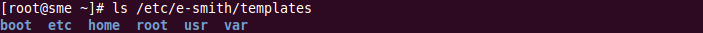
\includegraphics[width=\textwidth]{arquitectura/11templates.png}
\end{figure}

Aquí nos econtramos una estructura de directorios que se corresponde con la del sistema. Por ejemplo, la template para \lstinline!/etc/hosts! estará en \lstinline!/etc/e-smith/templates/etc/hosts!.\\

Las plantillas están almacenadas en \textbf{fragmentos}. Es decir, en nuestro ejemplo, \lstinline!/etc/e-smith/templates/etc/hosts! no es un archivo sino un directorio con diferentes archivos. Estos fragmentos se concatenan según el orden ASCII de sus nombres, y el archivo resultante es el que se encarga de generar el archivo de configuración de la aplicación.

\begin{figure}[H]
    \centering
    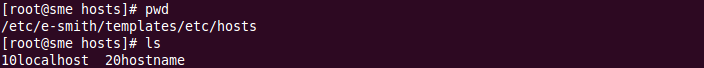
\includegraphics[width=\textwidth]{arquitectura/13hosts.png}
\end{figure}

La plantilla para \lstinline!/etc/hosts! es fácil de entender.

\begin{figure}[H]
    \centering
    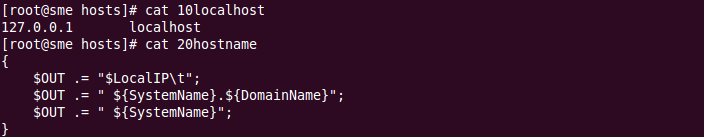
\includegraphics[width=\textwidth]{arquitectura/14hosts.png}
\end{figure}

El primer archivo contiene texto, que se añade sin más al archivo de configuración. El segundo archivo contiene un pequeño script de Perl (todo lo que va entre llaves se ejecuta), que usa valores de la base de datos de configuración.\\

\subsection{Expansión de templates}

Para regenerar los archivos de configuración cuya plantilla hemos modificado, debemos expandir esa plantilla:

\begin{lstlisting}
  expand-template /etc/archivo.conf
\end{lstlisting}

También debemos reiniciar el servicio en cuestión. Se puede hacer con el siguiente comando:

\begin{lstlisting}
  sv t /ruta/del/servicio
\end{lstlisting}

Algunos eventos combinan la expansión de ciertas plantillas y el reinicio de todos los servicios afectados. Por ejemplo, si modificamos algo en la configuración del email, llamaremos al siguiente evento:

\begin{lstlisting}
  signal-event email update
\end{lstlisting}

Si dudamos qué templates debemos expandir o qué servicios debemos reiniciar, podemos marcar los siguientes eventos, que expandirán todas las plantillas y reiniciarán el sistema:

\begin{lstlisting}
  signal-event post-upgrade
  signal-event reboot
\end{lstlisting}

\section{Ejemplo práctico: php.ini}

Si queremos modificar una de las templates o fragmentos que vienen presentes en la distribución, deberemos copiarla, junto con la estructura de directorios adecuada, desde \lstinline!/etc/e-smith/templates! a \lstinline!/etc/e-smith/templates-custom!, y editarla aquí. En caso de que exista una template en cada uno de estos dos directorios con el mismo nombre, solo se usará la de \lstinline!templates-custom!. Esto es así para que en el caso de que cometamos algún fallo podamos revertir el cambio fácilmente, sin más que borrar la plantilla en \lstinline!templates-custom!. Si queremos introducir una template nueva, la crearemos en \lstinline!templates-custom!, con el nombre adecuado, teniendo en cuenta que luego se concatenará con las demás (también las de \lstinline!/etc/e-smith/templates!) según el orden ASCII de sus nombres.\\

Veamos el aspecto que tiene el archivo \lstinline!/etc/php.ini! en el sistema:

\begin{figure}[H]
    \centering
    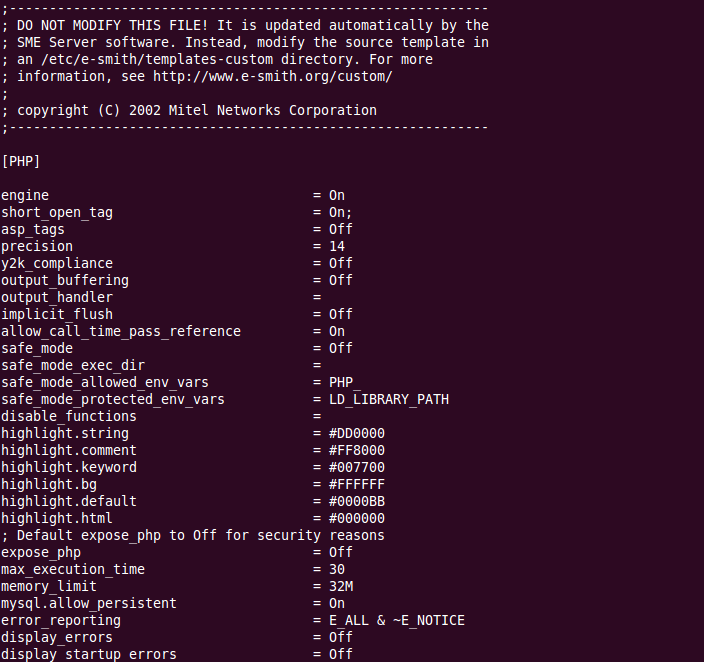
\includegraphics[width=\textwidth]{arquitectura/15phpIni.png}
\end{figure}

Supongamos que queremos cambiar el valor de la directiva \lstinline!display_errors! a \lstinline!On!. Debemos buscar la plantilla, dentro de \lstinline!/etc/e-smith/templates!, en la que se encuentra esta directiva.

\begin{figure}[H]
    \centering
    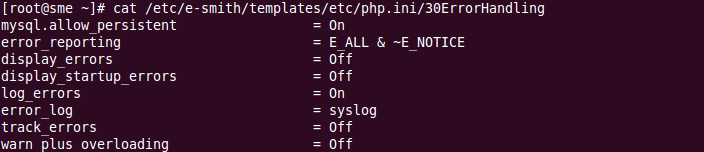
\includegraphics[width=\textwidth]{arquitectura/16.png}
\end{figure}

Copiamos este fragmento de plantilla en el directorio \lstinline!/etc/e-smith/templates-custom/etc/php.ini! (lo creamos si no existía) y lo modificamos allí, cambiando la directiva a \lstinline!On!. Así es como queda:

\begin{figure}[H]
    \centering
    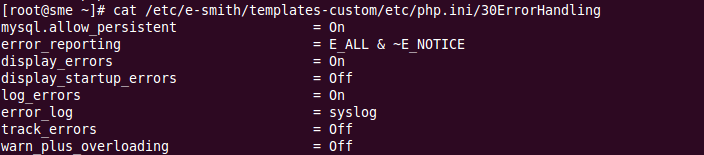
\includegraphics[width=\textwidth]{arquitectura/17.png}
\end{figure}

Para que se modifique el \lstinline!php.ini! real, tenemos que expandir la plantilla y reiniciar el servicio \lstinline!httpd-e-smith!, que es el servidor web.

\begin{lstlisting}
  expand-template /etc/php.ini
  sv t /service/httpd-e-smith
\end{lstlisting}

Podemos ver que el cambio se ha realizado correctamente:

\begin{figure}[H]
    \centering
    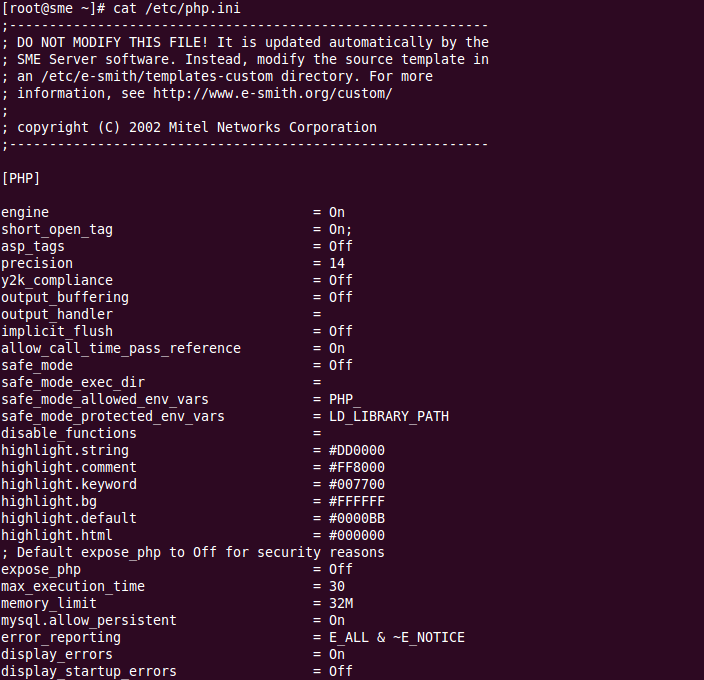
\includegraphics[width=\textwidth]{arquitectura/18.png}
\end{figure}


\chapter{Iptables}
Iptables es un programa que proporciona una interfaz de usuario para configurar Netfilter, que es el subsistema presente en el kernel de Linux para filtrado y manipulación de paquetes. Casi cualquier firewall de terceros que podemos descargar e instalar en Linux, como UFW o Firestarter, no son más que front-ends para Iptables.\\

Iptables es usado para crear y administrar reglas que proporcionan, entre otras cosas, capacidad para manipular los paquetes, control de la traducción NAT y seguimiento de conexiones. Iptables es un firewall de los llamados 'stateful', ya que mantiene el control de las conexiones establecidas por nuestro PC.

\section{Estructura y funcionamiento de iptables}
Iptables permite escribir \textbf{reglas} para control y manipulación de paquetes. Estas reglas se agrupan en \textbf{cadenas}, que a su vez pertenecen a una de las \textbf{tablas} presentes. \\

Las tablas disponibles son las siguientes:
\begin{itemize}
\item \textbf{Filter}, la tabla por defecto, provee comandos para filtar y aceptar o rechazar paquetes.
\item \textbf{Nat}, provee comandos para modificar la forma en que la máquina hace la traducción de direcciones.
\item \textbf{Mangle}, permite la modificación de los encabezamientos de los paquetes.
\item \textbf{Security}, proporciona reglas de control de acceso.
\item \textbf{Raw}, contiene herramientas para el seguimiento de conexiones.
\end{itemize}

Cada una de las tablas tiene diferentes cadenas, a las que añadiremos nuestras reglas:

\begin{longtable}{l | c}
\textbf{Tabla} \ \ \ & \textbf{Cadenas}\\\hline
\multirow{3}{*}{\textbf{filter}} & INPUT\\
& FORWARD\\
& OUTPUT\\\hline
\multirow{4}{*}{\textbf{NAT}} & PREROUTING\\
& INPUT\\
& OUTPUT\\
& POSTROUTING\\
\end{longtable}

\begin{longtable}{l | c}
\textbf{Tabla} & \textbf{Cadenas}\\\hline
\multirow{5}{*}{\textbf{mangle}} & PREROUTING\\
& INPUT\\
& FORWARD\\
& OUTPUT\\
& POSTROUTING\\\hline
\multirow{3}{*}{\textbf{security}} & INPUT\\
& FORWARD\\
& OUTPUT\\\hline
\multirow{2}{*}{\textbf{raw}} & PREROUTING\\
& OUTPUT\\
\end{longtable}

Para comprender bien el funcionamiento de Iptables debemos pensar desde el punto de vista de las cadenas en lugar de las tablas. El kernel de Linux procesa los paquetes en un orden que se corresponde con las cadenas. En esta imagen podemos ver las etapas por las que pasan los paquetes:

\begin{figure}[H]
    \centering
    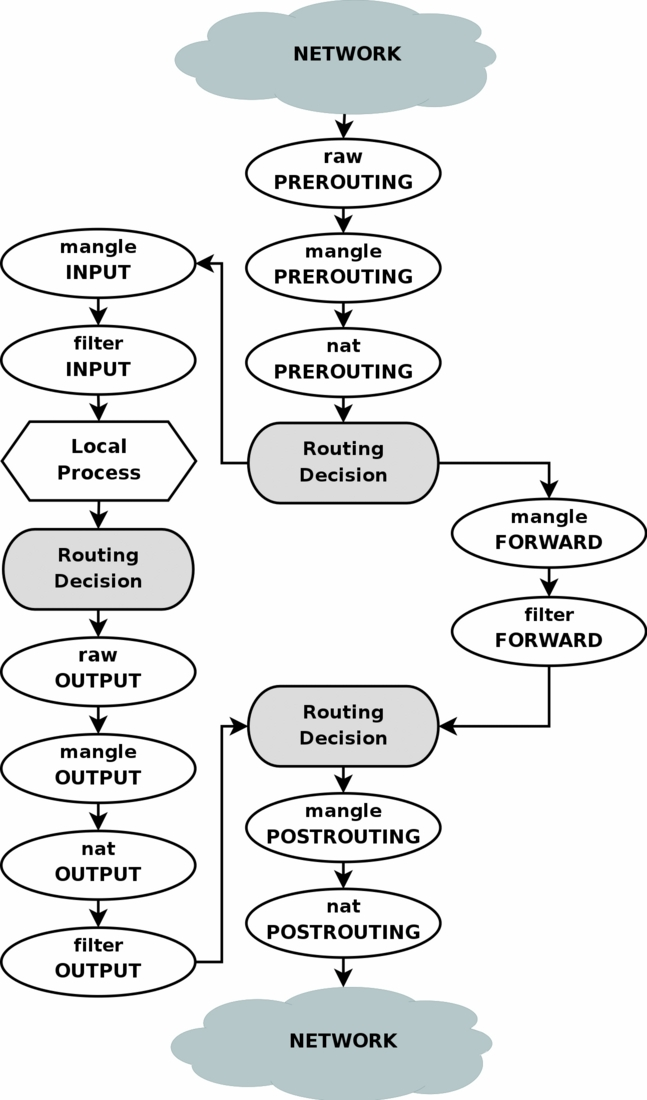
\includegraphics[width=0.55\textwidth]{iptables/00.jpg}
\end{figure}

Hay tres posibilidades diferentes según el camino que sigan los datos:

\begin{enumerate}[label=\bfseries\arabic*.]
\item \textbf{Paquetes destinados a nuestra máquina}

Cuando un paquete entra por una interfaz, inmediatamente se compara con las reglas que tengamos en la cadena PREROUTING, en el orden indicado en la imagen: primero las que están en la tabla \textit{raw}, luego las que están en la tabla \textit{mangle} y por último las que están en la tabla \textit{nat}. En este momento el paquete puede ser modificado. Por ejemplo, podemos cambiar la IP de destino y mandarlo a otro sitio, de manera que no será procesado por nuestro sistema. Se recomienda no usar nunca la cadena PREROUTING para filtrar, ya que en determinadas situaciones los paquetes no son filtrados correctamente.

Después, se toma la decisión de enrutamiento, con lo que se sigue el camino que vemos en la imagen hacia la izquierda. Se compara primero con la cadena INPUT de las tablas que la contienen. En este momento es cuando se filtran y modifican los paquetes. Finalmente se entrega al proceso local para que lo use.\\

\item \textbf{Paquetes generados por nuestra máquina}

Cuando el paquete se ha generado, se decide el enrutamiento y se elige qué dirección de origen usar y la interfaz por la que se va a enviar. Luego se compara con las reglas presentes en la cadena OUTPUT de las diferentes tablas. Con ellas podemos filtrar (tabla \textit{filter}) y cambiar las direcciones de origen y destino (tabla \textit{nat}), entre otras cosas.

Posteriormente se vuelve enrutar, ya que podríamos haber modificado el paquete, y se compara con las reglas de la cadena POSTROUTING. Finalmente se envía a la interfaz adecuada para que sea transmitido.\\

\item \textbf{Paquetes destinados a otro host}

En este caso el paquete entra y se compara con las reglas de la cadena PREROUTING, como hemos explicado antes, y luego se enruta. Si resulta que va dirigido a otro host, se compara con las reglas de la cadena FORWARD, en el orden indicado. Aquí podemos filtrar paquetes (tabla \textit{filter}) y modificarlos (tabla \textit{mangle}). Luego se vuelve a enrutar y se le aplican las reglas de la cadena POSTROUTING.

\end{enumerate}



\section{El comando iptables}

Veamos unos cuantos ejemplos para comprender la sintaxis:

\begin{lstlisting}
iptables -t nat -L
iptables -L
iptables -t nat -L PREROUTING
\end{lstlisting}

El primer comando muestra las reglas presentes en la tabla \textit{nat}. La tabla por defecto es \textit{filter}, por lo tanto se usará ésta siempre que no se especifque otra: el segundo ejemplo mostrará todas las reglas presentes en \textit{filter}. Se puede añadir el nombre de una cadena después para que solo muestre las reglas contenidas en ella.

\begin{figure}[H]
    \centering
    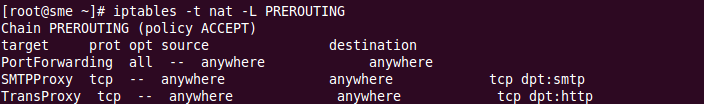
\includegraphics[width=\textwidth]{iptables/01.png}
\end{figure}

\begin{lstlisting}
iptables -t mangle -F INPUT
\end{lstlisting}

Borra todas las reglas de la cadena INPUT de la tabla \textit{mangle}. Si se omite el nombre de la tabla, se utilizará \textit{filter}. Si se omite el nombre de la cadena, se borrarán las reglas de todas las cadenas.\\

\begin{lstlisting}
iptables -t filter -P INPUT DROP
\end{lstlisting}

Cambia la política por defecto de la cadena INPUT de la tabla \textit{filter} a DROP. Los paquetes que se hayan comparado con todas las reglas de esta cadena y no se hayan encontrado con una orden ACCEPT serán rechazados.\\

\begin{lstlisting}
iptables -t nat -N miCadena
\end{lstlisting}

Crea una nueva cadena definida por el usuario, llamada \textit{miCadena}, en la tabla \textit{nat}. Estas cadenas deben ser llamadas desde las 5 originales, más adelante veremos cómo.

\subsection{Añadiendo reglas}

El comando básico para añadir una regla a una cadena de una tabla es

\begin{lstlisting}
iptables -t tabla -A CADENA descripición
\end{lstlisting}

La descripción de una regla se especifica escribiendo el valor de varios parámetros. Los parámetros disponibles son:

\begin{longtable}{p{0.21\textwidth} | p{0.7\textwidth}}
\textbf{Parámetro} & \textbf{Descripción}\\\hline
\lstinline!-p! \textit{protocolo} & Especifica el protocolo. Puede ser \textit{tcp}, \textit{udp} o \textit{icmp}, entre otros. Se puede usar un símbolo de exclamación, !, delante del protocolo para invertir la búsqueda.\\\hline
\lstinline!-s! \textit{IP/máscara} & Especificación del origen. Puede ser un nombre de host en lugar de una dirección IP. Se pueden poner varias separadas por coma. Se puede usar ! para invertir la búsqueda.\\\hline
\lstinline!-d! \textit{IP/máscara} & Dirección IP o nombre de host del destino.\\\hline
\lstinline!-m! \textit{parámetros} & Con \lstinline!-m! o \lstinline!--match! podemos dar condiciones más detalladas del paquete. Si las cumple, se ejecutará la acción en la opción \lstinline!-j!. Más abajo se dará una lista con los parámetros disponibles.\\\hline
\lstinline!-j! \textit{target} & Especifica qué hacer cuando el paquete cumple todas las condiciones establecidas en la regla. Los targets básicos son REJECT, DROP, ACCEPT y LOG. Algunos aceptan opciones extra. También se puede poner el nombre de una cadena personalizada, con lo que se pasará a comparar el paquete con todas las reglas de esa cadena.\\\hline
\lstinline!-i! \textit{interfaz} & Nombre de la inerfaz desde la que se ha recibido un paquete. Slo disponible en las cadenas INPUT, FORWARD y PREROUTING. Se puede usar ! al principio para revertir la búsqueda, o + al final como carácter comodín.\\\hline
\lstinline!-o! \textit{interfaz} & Nombre de la interfaz por la que el paquete va a ser enviado. Solo disponible en las cadenas FORWARD, OUTPUT y POSTROUTING. Se puede usar ! al principio para revertir la búsqueda, o + al final como carácter comodín.\\
\end{longtable}

Con la opción \lstinline!-m! debemos usar lo que se llaman \textbf{módulos} de filtrado. Cada módulo tiene un nombre y acepta diferentes opciones, que se pueden escribir en la misma línea. Algunos de ellos son:

\begin{longtable}{p{0.13\textwidth} | p{0.29\textwidth} | p{0.49\textwidth}}
\textbf{Módulo} &  \textbf{Opciones} & \textbf{Descripción}\\\hline
\lstinline!state! & \lstinline!--state! \textit{estado} & Comprueba el estado de conexión de ese paquete. El estado puede ser INVALID (no hay ninguna conexión conocida asociada a ese paquete), NEW (el paquete ha empezado una nueva conexión) y ESTABLISHED (el paquete está asociado a una conexión conocida, que ya ha enviado paquetes en ambos sentidos), entre otros.\\\hline
\lstinline!limit! & \lstinline!--limit! \textit{núm/ud\_tiempo} \quad \lstinline!--limit-burst! \textit{número} & La regla en la que está \lstinline!limit! se comprobará como máximo una vez en el intervalo de tiempo que le digamos. \lstinline!/s, /m, /h, /d! para segundos, minutos, horas y días. \lstinline!--limit-burst! marca el número de veces que se permiten antes de que el límite sea efectivo. Después de una regla con \lstinline!limit! se suele usar una con DROP, para descartar el resto de paquetes.\\\hline
\lstinline!tcp! & \lstinline!--sport! \textit{puerto[:puerto]} \lstinline!--dport! \textit{puerto[:puerto]} \hspace{2cm} \lstinline!--tcp-flags! \textit{flags} \textit{flags}
\lstinline!--syn! & Se pueden usar estas opciones directamente detrás de \lstinline!-p tcp! en una regla. Permite filtrar un paquete según su puerto de origen y destino (se pueden usar rangos), y según su tipo, dependiendo de las flags TCP que tenga. El primer parámetro en \lstinline!--tcp-flags! es para las flags que deben ser examinadas y el segundo para las que deben estar activadas, es decir las que estén en el primer parámetro y no en el segundo deberán estar sin activar. \lstinline!--syn! es equivalente a \lstinline!--tcp-flags SYN,RST,ACK,FIN SYN!\\
\end{longtable}

\newpage
Veamos algunos ejemplos sencillos de reglas:\\

\begin{lstlisting}
iptables -A INPUT -s 192.168.0.0/24 -j DROP
\end{lstlisting}

Descarta los paquetes que vengan desde la red 192.168.0.0/24 por cualquier interfaz. La diferencia entre los targets DROP y REJECT es que este último envía de vuelta un mensaje ICMP de destino inalcanzable (podemos cambiar este mensaje con la opción \hspace{0.7cm} \lstinline!--reject-with!), mientras que DROP lo bloquea sin más.\\

\begin{lstlisting}
iptables -A INPUT -i eth0 -p tcp -s 192.168.0.0/24 --dport 22 -m state NEW, ESTABLISHED -j ACCEPT
iptables -A OUTPUT -o eth0 -p tcp --sport 22 -m state --state ESTABLISHED -j ACCEPT
\end{lstlisting}

Permite todo el tráfico SSH que provenga de la red 192.168.0.0/24, siempre que haya iniciado la conexión otro host (esto último depende de la política por defecto que hayamos puesto en OUTPUT, suponemos que es DROP).\\

\begin{lstlisting}
iptables -t nat -A POSTROUTING -o eth0 -j MASQUERADE
iptables -A FORWARD -i eth0 -o eth1 -m state --state RELATED,ESTABLISHED -j ACCEPT
iptables -A FORWARD -i eth1 -o eth0 -j ACCEPT
\end{lstlisting}

Estas son las reglas necesarias para hacer traducción de direcciones. eth0 sería la interfaz externa y eth1 la interna. La primera regla es para que nuestra máquina enmascare el tráfico que sale hacia el exterior, es decir, que haga la traducción de direcciones para que parezca que el paquete ha sido enviado por ella. La segunda es para permitir todo el tráfico hacia las máquinas de la red interna, siempre que hayamos iniciado nosotros la comunicación. Está en la cadena FORWARD de la tabla \textit{filter}, con lo cual en el momento de comprobar esta regla ya se ha hecho el enrutamiento y la dirección de destino será una de nuestra red interna. La tercera regla sirve para permitir todo el tráfico desde nuestra red interna al exterior.

%BIBLIOGRAFIAA
%http://www.thegeekstuff.com/2011/06/iptables-rules-examples/
%https://help.ubuntu.com/community/IptablesHowTo
%http://gr8idea.info/os/tutorials/security/iptables8.html
%https://www.digitalocean.com/community/tutorials/iptables-essentials-common-firewall-rules-and-commands
%


\chapter{El firewall de SME Server}
El firewall de SME server es modificado automáticamente en respuesta a los cambios que hacemos en la configuración, como activar o desactivar servicios, hacerlos públicos o privados o reenviar puertos.\\

Por ejemplo, si añadimos una regla de reenvío de puertos en la interfaz web:

\begin{figure}[H]
    \centering
    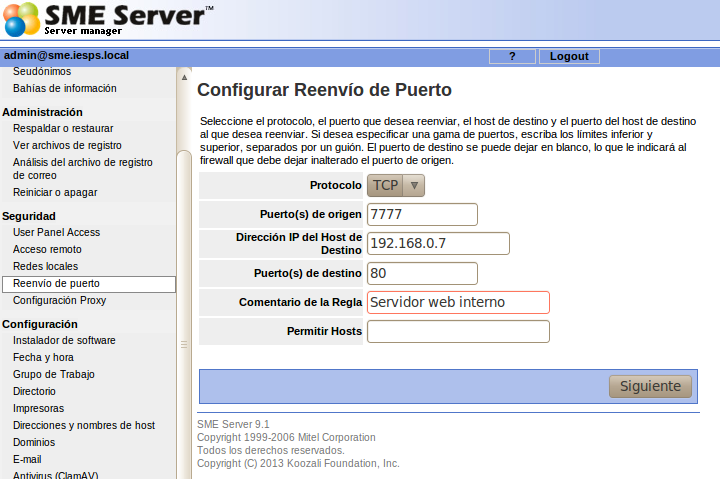
\includegraphics[width=\textwidth]{firewall/00.png}
\end{figure}

Podemos ver cómo la regla se ha añadido a la tabla \textit{nat}.

\begin{figure}[H]
    \centering
    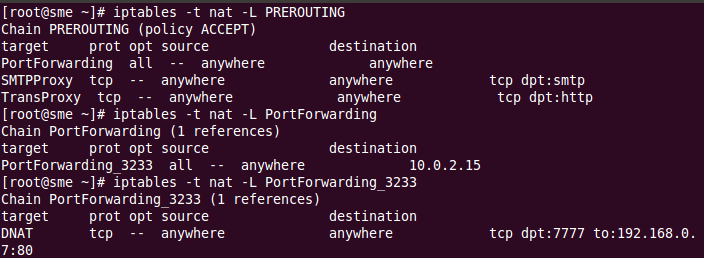
\includegraphics[width=\textwidth]{firewall/01.png}
\end{figure}

Primero consultamos la cadena PREROUTING de la tabla \textit{nat}, que es donde se tienen que añadir las reglas de Iptables para traducción de direcciones. Vemos que hay un target de nombre PortForwarding. Al no ser un target estándar de Iptables, se refiere a una cadena personalizada que el servidor ha creado. Como no tiene filtro, todos los paquetes serán pasados por esa cadena. La consultamos y vemos que a todos los paquetes que entren con IP destino 10.0.2.15 (la externa del servidor), les aplicará el target PortForwarding\_3233, que es otra cadena personalizada. Finalmente consultamos esta y vemos que está la regla que hace DNAT (en este caso se refiere a Destination NAT, cambio de la dirección de destino).\\

Hay dos formas en las que podemos hacer una configuración más avanzada del firewall: modificando ciertos valores en la base de datos para los distintos servicios o creando templates propias para cambiar directamente la configuración de Iptables.

\section{Modificación del firewall}

El archivo responsable de cargar toda la configuración de Iptables en el sistema es \lstinline!/etc/rc.d/init.d/masq!, por tanto las plantillas se encuentran en \lstinline!/etc/e-smith/templates/etc/rc.d/init.d/masq!.

\begin{figure}[H]
    \centering
    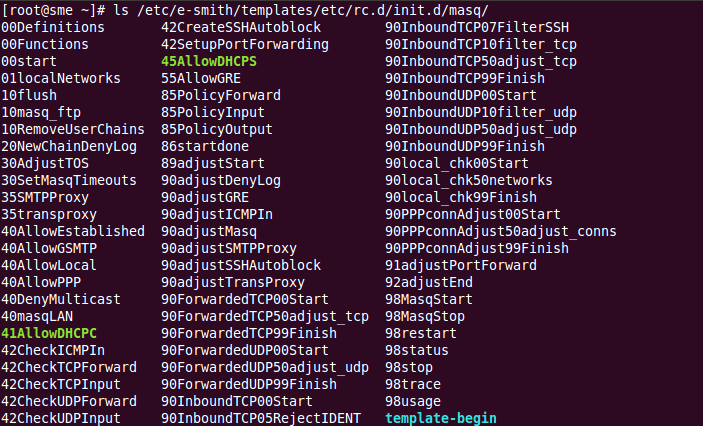
\includegraphics[width=\textwidth]{firewall/05.png}
\end{figure}

Tendremos que copiar y modificar la plantilla adecuada en \lstinline!templates-custom!, o crear una nueva, y luego expandirla con \lstinline!expand-template! y reiniciar el servicio: \lstinline!/etc/init.d/masq restart!. \\

Vamos a configurar el firewall del servidor para proporcionar una seguridad más fuerte en el caso de algunos ataques comunes:

\subsection{Denegación de servicio}

Un ataque de denegación de servicio (denial-of-service, DoS) causa que un servicio o recurso sea inaccesible a sus usuarios. Se suelen generar mediante la saturación de los puertos con flujo de información, consumiendo todo el ancho de banda y bloqueando así el servidor. Existen diferentes tipos de ataques de denegación de servicio por lo que hay que elaborar una respuesta para cada uno de ellos.\\

\begin{itemize}
\item \textbf{Ping flood}
\end{itemize}

Consiste en saturar al servidor con paquetes ICMP, enviándolos lo más rápido posible sin esperar respuesta. Esto provoca que se consuma mucho ancho de banda de entrada y también de salida, puesto que el servidor intentará responder. Es más efectivo si el ancho de banda disponible para el atacante es mayor que el del servidor.\\

Para comprobar si SME server está configurado contra el ping flood por defecto, le he cambiado el adaptador en VirtualBox a modo bridge, para que la interfaz externa esté en la misma red que mi ordenador (la nueva IP es 192.168.1.250), y le he atacado desde ahí. Todos los pings son satisfactorios con lo que SME no está protegido contra esto.

\begin{figure}[H]
    \centering
    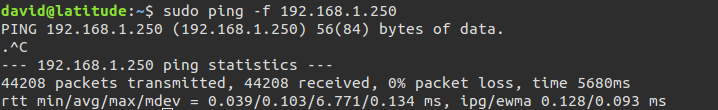
\includegraphics[width=\textwidth]{firewall/07.png}
\end{figure}

Una solución para evitar esto es permitir solamente un ping por segundo. Podemos escribir una nueva cadena para controlar esto y llamarla desde INPUT cuando se encuentren paquetes ICMP.

\begin{lstlisting}
/sbin/iptables -N icmpFlood
/sbin/iptables -A icmpFlood -p icmp --icmp-type echo-request -m limit --limit 1/s --limit-burst 1 -j ACCEPT
/sbin/iptables -A icmpFlood -j DROP

/sbin/iptables -A INPUT -p icmp -j icmpFlood
\end{lstlisting}

En este caso usaré la plantilla 39misReglas, para que la regla que está en la cadena INPUT se añada al principio. Las cadenas en la tabla \textit{filter} quedan así:

\begin{figure}[H]
    \centering
    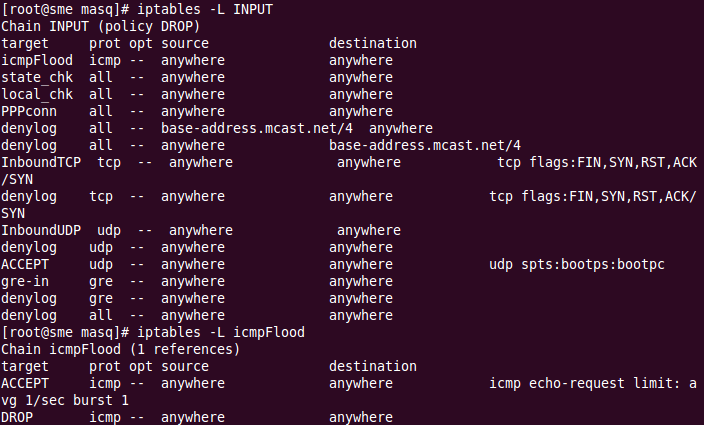
\includegraphics[width=\textwidth]{firewall/17.png}
\end{figure}

Con estas reglas se soluciona el problema. Este es el resultado al volver a intentar el ping flood desde nuestro ordenador:

\begin{figure}[H]
    \centering
    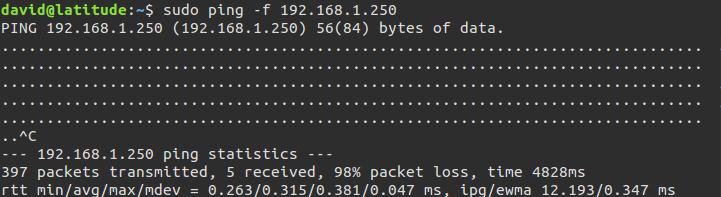
\includegraphics[width=\textwidth]{firewall/13buena.png}
\end{figure}
\vspace{0.15cm}
\begin{itemize}
\item \textbf{SYN flood}
\end{itemize}

Cuando queremos iniciar una conexión TCP, se produce el saludo a tres vías: el cliente envía un mensaje con la bandera SYN, el servidor responde con un mensaje SYN-ACK y finalmente el cliente responde con un mensaje ACK. El ataque SYN flood consiste en saturar el servidor mandando mensajes SYN y no respondiendo con los correspondientes ACK.\\

En Linux podemos usar el programa hping3 con este fin.

\begin{figure}[H]
    \centering
    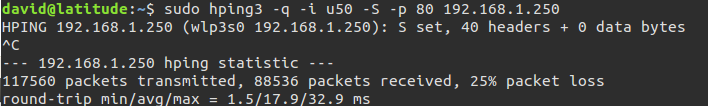
\includegraphics[width=\textwidth]{firewall/16syn.png}
\end{figure}

Con el comando de la imagen enviamos un mensaje con la bandera SYN al puerto 80 cada 50 microsegundos. Como resultado, mientras se está ejecutando este comando el servidor está bloqueado, impidiéndonos por ejemplo acceder a la interfaz web de administración.\\

Para solucionarlo de una forma distinta al anterior, se puede utilizar el módulo \lstinline!recent!:

\begin{lstlisting}
modprobe ipt_recent

/sbin/iptables -N synFlood
/sbin/iptables -A synFlood -m recent --set
/sbin/iptables -A synFlood -m recent --update --seconds 2 --hitcount 20 -j DROP

/sbin/iptables -A INPUT -p tcp --tcp-flags SYN SYN -j synFlood
\end{lstlisting}

La primera línea es para cargar el módulo. La última es para que los paquetes que tengan al menos la bandera SYN pasen por nuestra cadena synFlood. La primera regla de la nueva cadena añade la IP de origen del paquete a la lista. Si ya está en la lista, actualiza la entrada. La siguiente línea se encarga de actualizar el tiempo en el que se ha visto esa IP y rechazar los paquetes si la IP ha sido vista en la tabla en los últimos dos segundos y si tiene al menos 20 paquetes enviados. La lista que guarda los paquetes enviados no tiene en cuenta el tiempo en el que han llegado. Esto quiere decir que el control solo se reiniciará cuando la IP de origen haya estado 2 segundos sin enviar ningún paquete, o al menos ninún paquete que se haya comparado contra esta regla. Como podemos ver, ahora solo llegan 19 paquetes de vuelta:

\begin{figure}[H]
    \centering
    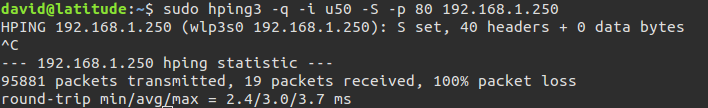
\includegraphics[width=\textwidth]{firewall/18.png}
\end{figure}

\subsection{Suplantación de identidad}

Este tipo de ataque consiste en que un host o aplicación se hace pasar por otro. Por ejemplo, nos pueden llegar paquetes desde la interfaz externa con IPs de nuestra red interna. En estos casos el atacante no se preocupa de la respuesta que origina el paquete ya que no le llegará.\\

Podemos lanzar un ataque SYN flood de manera que cada paquete que enviemos se envíe con una dirección IP de origen aleatoria, con lo que la regla que hemos creado contra estos ataques no serviría para nada. El programa hping3 permite hacerlo de manera sencilla, sin más que añadir la opción \lstinline!--rand-source!:

\begin{figure}[H]
    \centering
    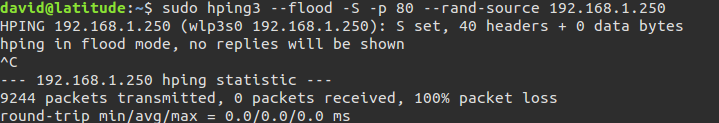
\includegraphics[width=\textwidth]{firewall/21.png}
\end{figure}

Estamos provocando que nuestro servidor mande mensajes SYN-ACK a esas IPs aleatorias.

\begin{figure}[H]
    \centering
    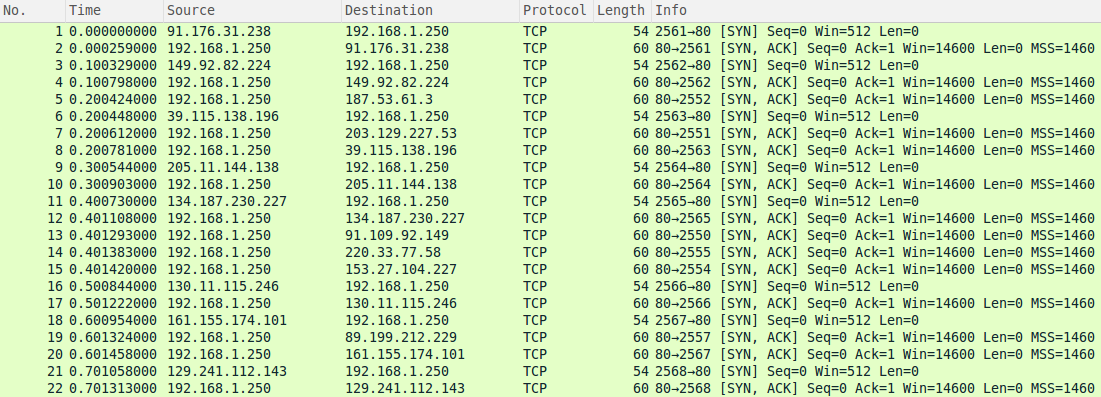
\includegraphics[width=\textwidth]{firewall/22.png}
\end{figure}

\newpage

Esto puede ser evitado con una regla de las del primer tipo, la que vimos para el ping flood.

\begin{lstlisting}
/sbin/iptables -N synFlood2
/sbin/iptables -A synFlood2 -m limit --limit 1/s --limit-burst 1 -j RETURN
/sbin/iptables -A synFlood2 -j DROP

/sbin/iptables -A INPUT -p tcp --tcp-flags SYN SYN -j synFlood2

/sbin/iptables -A INPUT -s 10.0.0.0/8 -i eth0 -j DROP
/sbin/iptables -A INPUT -s 172.16.0.0/12 -i eth0 -j DROP
/sbin/iptables -A INPUT -s 192.168.0.0/16 -i eth0 -j DROP
/sbin/iptables -A INPUT -s 224.0.0.0/4 -i eth0 -j DROP
/sbin/iptables -A INPUT -s 240.0.0.0/5 -i eth0 -j DROP
/sbin/iptables -A INPUT -s 127.0.0.0/8 -i eth0 -j DROP
/sbin/iptables -A FORWARD -s 10.0.0.0/8 -i eth0 -j DROP
/sbin/iptables -A FORWARD -s 172.16.0.0/12 -i eth0 -j DROP
/sbin/iptables -A FORWARD -s 192.168.0.0/16 -i eth0 -j DROP
/sbin/iptables -A FORWARD -s 224.0.0.0/4 -i eth0 -j DROP
/sbin/iptables -A FORWARD -s 240.0.0.0/5 -i eth0 -j DROP
/sbin/iptables -A FORWARD -s 127.0.0.0/8 -i eth0 -j DROP

\end{lstlisting}

También hemos añadido varias reglas para rechazar paquetes que vengan desde la interfaz eth0, que es la de la red externa, con dirección IP de origen de una red privada, de multicast o de loopback. Podemos comprobar que las reglas contra el SYN flood son efectivas analizando el tráfico y viendo que solo hay una respuesta SYN-ACK del servidor cada segundo.

\begin{figure}[H]
    \centering
    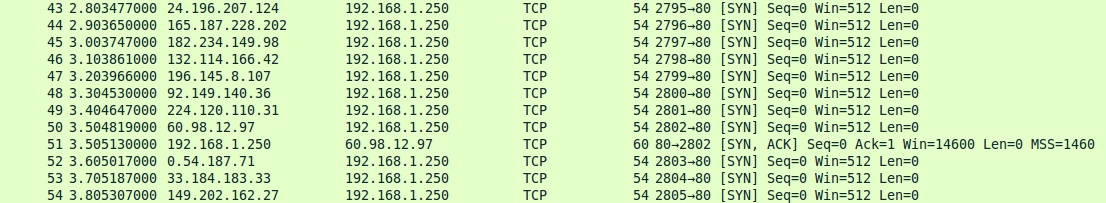
\includegraphics[width=\textwidth]{firewall/23.png}
\end{figure}

%\begin{longtable}{p{0.21\textwidth} | p{0.7\textwidth}}
%\textbf{Parámetro} & \textbf{Descripción}\\\hline
%\end{longtable}

%BIBLIOGRAFIAA
%https://wiki.contribs.org/Firewall
%http://blog.desdelinux.net/ddos-y-otros-ataques-vs-iptables-seguridad-anti-ddos-en-iptables/
%http://es.tldp.org/Manuales-LuCAS/GARL2/garl2/index.html
%http://www.cyberciti.biz/tips/linux-iptables-examples.html




%\chapter{Conclusión}
%\input{chapters/conclusion}

%\appendix
%\chapter{Apéndice}
%\input{chapters/apendice}

% Bibliografia
%\nocite{*}
%\printbibliography

\newpage
\thispagestyle{plain}
\begin{center}
\Huge
\textbf{Bibliografía}
\end{center}\vspace{0.3cm}

\begin{itemize}
\item \textbf{Manuales de SME Server}\\
https://wiki.contribs.org/SME\_Server:Documentation:Administration\_Manual\\
https://wiki.contribs.org/SME\_Server:Documentation:Developers\_Manual\\
https://wiki.contribs.org/Template\_Tutorial\\

\item \textbf{Manuales de Iptables}\\
http://www.tony-hill.info/app/download/1367500/IPTABLES+Tutorial+V1-3.pdf\\
https://www.frozentux.net/iptables-tutorial/iptables-tutorial.html\\
http://es.tldp.org/Manuales-LuCAS/doc-iptables-firewall/doc-iptables-firewall.pdf\\

\item \textbf{Otros recursos y ejemplos}\\
http://es.tldp.org/Manuales-LuCAS/GARL2/garl2/index.html\\
https://help.ubuntu.com/community/IptablesHowTo\\
http://www.cyberciti.biz/tips/linux-iptables-examples.html\\
http://www.thegeekstuff.com/2011/01/iptables-fundamentals/\\
http://blog.desdelinux.net/ddos-y-otros-ataques-vs-iptables-seguridad-anti-ddos-en-iptables/
\end{itemize}


\end{document}
% Cambio de nombres de cosass
% http://tex.stackexchange.com/questions/82993/how-to-change-the-name-of-document-elements-like-figure-contents-bibliogr
% Nombres de capitulo
% http://texblog.org/2012/07/03/fancy-latex-chapter-styles/
% Bibliografia
% https://www.sharelatex.com/learn/Bibliography_management_in_LaTeX
% Tutorial
% https://www.sharelatex.com/blog/2013/08/06/thesis-series-pt2.html
